\documentclass{article}

\usepackage{amsmath, amsthm}
\usepackage{setspace}
\usepackage{microtype, parskip}
\usepackage[comma,sort&compress]{natbib}
\usepackage{lineno}
\usepackage{docmute}
\usepackage{caption, subcaption, multirow, morefloats, rotating}
\usepackage{wrapfig}

\frenchspacing

\doublespacing

\raggedright

\begin{document}
\linenumbers
\modulolinenumbers[2]

%\maketitle

\begin{titlepage}
  \begin{large}
    \textbf{Title:} How do biological traits affect brachiopod taxonomic survival? A hierarchical Bayesian approach.
  \end{large}

  \textbf{Running title:} How do biological traits affect taxonomic survival?

  \textbf{Author:} Peter D Smits, psmits@uchicago.edu, Committee on Evolutionary Biology, University of Chicago

  \textbf{Keywords:} extinction, macroevolution, macroecology, Paleozoic, selection

  \textbf{Word count:} ?
  
  \textbf{Table count:} 0.
 
  \textbf{Figure count:} 9 main text, 3 supplement.

  \textbf{Data archival location:} If accepted, all data and code necessary to duplicate this analysis will be made available on DRYAD.

\end{titlepage}

\documentclass[12pt,letterpaper]{article}

\usepackage{amsmath, amsthm}
\usepackage{microtype, parskip}
\usepackage[comma,numbers,sort&compress]{natbib}
\usepackage{lineno}
\usepackage{docmute}
\usepackage{caption, subcaption, multirow, morefloats, rotating}
\usepackage{wrapfig}

\frenchspacing

\captionsetup[subfigure]{position = top, labelfont = bf, textfont = normalfont, singlelinecheck = off, justification = raggedright}

\begin{document}

\begin{abstract}
  Write me.
\end{abstract}

\end{document}


\documentclass[12pt,letterpaper]{article}

\usepackage{amsmath, amsthm}
\usepackage{microtype, parskip}
\usepackage[comma,numbers,sort&compress]{natbib}
\usepackage{lineno}
\usepackage{docmute}
\usepackage{caption, subcaption, multirow, morefloats, rotating}
\usepackage{wrapfig}

\frenchspacing

\captionsetup[subfigure]{position = top, labelfont = bf, textfont = normalfont, singlelinecheck = off, justification = raggedright}

\begin{document}
\section{Introduction}

% precision of question
%   how does taxonomic entrance and loss contribute to regional/latitudinal diversity? 
%   how do regions compare in terms of how diversity accumulates?
The spatial context of how taxonomic diversity changes over time

% latitudinal diversity gradients
%   hypotheses as to why, in terms of diversification

% Phanerozoic brachiopods
%   previous work on diversification
%   LDG

Key to this study is the idea that any given taxon might leave a region and then re-enter it at a later time. This fact means that standard approaches which assume constant/range-through presence following initial occurrence until final occurrence \citep{Alroy2010c,Foote2003,Foote2000,Foote2000a,Smits2015,Liow2008,Liow2015,Silvestro2014a} are inappropriate as they do not capture the macroevolutionary process of interest. Additionally, given the imperfect record that is the fossil record, distinguishing between true absence and unobserved presence becomes an extremely goal when trying to understand the macroevolutionary processes of interest here.

Here I choose to model regional diversity as a hidden Markov Model (HMM), which is how occupancy is modeled in ecology \citep{Royle2008}. In a HMM, the observed state of an individual is considered imperfectly observed, such that actually observing the ``true'' or latent state is done with some sampling probability. The actual diversification process affects the latent state of a taxon, which is itself estimated. A HMM is similar to a Jolly-Seber capture-mark-recapture model \citep{Liow2015,Royle2008} except the transition from 1 to 0 is not an absorbing state and taxa can ``return to life.''


\end{document}


\documentclass[12pt,letterpaper]{article}

\usepackage{amsmath, amsthm}
\usepackage{microtype, parskip}
\usepackage[comma,numbers,sort&compress]{natbib}
\usepackage{lineno}
\usepackage{docmute}
\usepackage{caption, subcaption, multirow, morefloats, rotating}
\usepackage{wrapfig}

\frenchspacing

\begin{document}
\section{Methods}

\subsection{Fossil occurrence information}

The dataset analyzed here is derived from the a combination of the occurrence information from \citet{Miller2009a} and the body size data from \citet{Payne2014}. The \citet{Miller2009a} dataset is based on the Paleobiology Database (http://www.paleodb.org); see \citet{Miller2009a} for a full description of the inclusion criterion. 

Sampled occurrences were restricted to those with latitude and longitude coordinates, assignment to either epicontinental or open-ocean environment, and being of a genus present in the body size dataset. Genus duration was calculated as the number of geologic stages from first appearance to last appearance, inclusive. Genera who's last appearance was in a stage preceding a mass extinction were right censored, and genera with a duration of only one stage and were left censored (see below for explanation of censoring). The covariates used to model genus duration were geographic range size (\(r\)), environmental preference (\(v\)), and body size (\(m\)). 

Geographic range was calculated using an occupancy approach. First, all occurrences were projected onto an equal-area cylindrical map projection. Each occurrence was then assigned to one of the cells of a 70 \(\times\) 34 regular raster grid placed on the map. Each grid cell represents approximately 250,000 km\(^{2}\). Following this, for each stage, the total number of grid cells occupied is calculated. The number of grid cells that each genus present occurs in was then calculated and made relative by dividing by the total number of possible cells. Finally, mean relative genus occupancy was calculated as the mean of per stage relative occupancy.

Body size data was sourced directly from \citet{Payne2014}. Because those measurements are presented with out quantified error, a measurement error model similar to the one for environmental affinity could not be implemented.

Prior to analysis some covariates were transformed in order to improve interpretation. Geographic range size, which can only have between 0 and 1, was logit transformed. Body size, which is defined for all positive real values was natural log transformed. These covariates were then standardized by mean centering and dividing by two times their standard deviation following \citet{Gelman2007}.

\subsubsection{Uncertainty in environmental preference}
The calculation and inclusion of environmental affinity in the subsequent survival model is a statistical procedure that takes into account our uncertainty based on where fossils tend to occur. Because we cannot directly observe if a fossil taxon had occurrences restricted to only a single environmental, instead we can only get an of affinity with some amount of uncertainty. One advantage of using a Bayesian analytical context is that both parameters and data are considered random samples from some underlying distribution, which means it is possible to model the uncertainty in our covariates of interest \citep{Gelman2013d}. In this case, this is the genus affnity to either epicontiental settings or not. This approach is conceptually similar to \citet{Simpson2009} but instead of obtaining a single point estimate, an entire posterior distribution is estimated.

The first step is to determine the probability \(\theta\) at which genus \(i\) occurs in an epicontinental settings based on its own pattern of occurrences. Define \(e_{i}\) as the number of occurrences of genus \(i\) in an epicontiental sea and \(o_{i}\) as the number of occurrences of genus \(i\) not in an epicontinental sea (e.g. open ocean). Because the value of inters is the probability of occurring in an epicontinental environment, given the observed fossil record, I assume that probability follows a beta distribution. We can then define our sampling statement as
\begin{equation}
  e_{i} \sim \mathrm{Binomial}(e_{i} + o_{i}, \theta_{i}).
  \label{eq:epi_lik}
\end{equation}
I used a flat prior of \(\theta_{i}\) defined as \(\theta_{i} \sim \mathrm{Beta}(1, 1)\). Because the beta distribution is the conjugate prior for the binomial distribution, the posterior is easy to compute in closed form. The posterior probability of \(\theta\) is then 
\begin{equation}
  \theta_{i} \sim \mathrm{Beta}(e_{i} + 1, o_{i} + 1)
  \label{eq:epi_post}
\end{equation}

It is extremely important, however, to take into account the overall environmental occurrence probability of all other genera present at the same time as genus \(i\). This is incorporated as an additional probability \(\Theta\). Define \(E_{i}\) as the total number of other fossil occurrences (e.g. excepting for genus \(i\)) in epicontinental seas during stages where \(i\) occurs and \(O_{i}\) as the number of other fossil occurrences not on epicontinental seas. We can then define the sampling statement as
\begin{equation}
  E_{i} \sim \mathrm{Binomial}(E_{i} + O_{i}, \Theta_{i}).
  \label{eq:bck_lik}
\end{equation}
Again, I used a flat prior of \(\Theta_{i}\) defined as \(\Theta_{i} \sim \mathrm{Beta}(1, 1)\). The posterior of \(\Theta\) is then simply defined as
\begin{equation}
  \Theta_{i} \sim \mathrm{Beta}(E_{i} + 1, O_{i} + 1)
  \label{eq:bck_post}
\end{equation}

I then define the environmental affinity of genus \(i\) as \(v_{i} = \theta_{i} - \Theta_{i}\). \(v_{i}\) is a value that can range between -1 and 1, where negative values indicate that genus \(i\) tends to occur in open ocean environments while positive values indicate that genus \(i\) tends to occur in epicontiental environments.

While this approach is noticeably more complicated than previous ones \citep{Foote2006,Miller2001,Simpson2009,Kiessling2007a} there are some important benefits to both using a continuous measure of affinity as well directly modeling our uncertainty. In order to show case some of these benefits, I performed a simulation analysis of how modal/maximum \textit{a posteriori}(MAP) estimates versus full posterior estimates.

In this simulation, I first defined the ``background'' epicontinental occurrence \(\theta_{b}\) as 0.50 with a small amount of noise. This was represented as a beta distribution 
\begin{equation}
  \theta_{b} = \mathrm{Beta}(\alpha = 2500, \beta = 2500). 
  \label{eq:bck_sim}
\end{equation}
This choice of parameters for the distribution reflects the average number of background occurrences for either epicontinental or open ocean environments per genus.

Using this background occurrence ratio, randomly generated the occurrence patterns 1000 simulated taxa. This was done at multiple sample sizes (1, 2, 3, 4, 5, 10, 25, 50, 100) in order to demonstrate the effects of increasing sample size on the confidence of environmental affinity. For each simulated taxon I calculated the full posterior distribution while assuming a flat Beta prior (\(\mathrm{Beta}(1, 1)\)). Using the full posterior I calculated the MAP probability of occurring in epicontinental environments. The environmental affinity was calculated for each of the simulated taxa using both the full posterior and the MAP estimate. In this toy example, environmental affinity can range between -0.5 and 0.5.

As should be expected, as sample size increases the distribution of MAP estimates converge on the true value (Fig. \ref{fig:env_mode}). For taxa with less than 10 occurrences, the MAP estimate is biased towards over estimates of affinity.
\begin{figure}[ht]
  \centering
  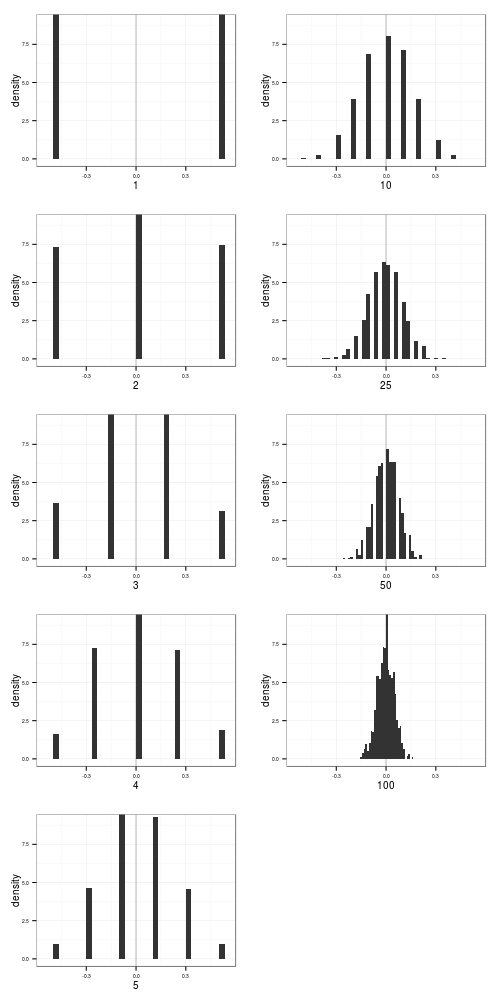
\includegraphics[height = \textheight,width=\textwidth,keepaspectratio=true]{figure/env_mode_dist}
  \caption{<+caption text+>}
  \label{fig:env_mode}
\end{figure}

In contrast, we can compare the true occurrence probability distribution versus the posterior estimate for a given sample (Fig. \ref{fig:env_post}). When sample sizes are low, posterior estimates are flat and represent a compromise between the likelihood (equivalent to MAP) and the flat prior. Because of this, estimates from small sizes are less likely to be overly biased. This is further emphasized by inspection of the estimates of environmental affinity for the simulated taxa (Fig. \ref{fig:env_diff}). Posterior estimates from simulated taxa with small sample size have a much broader distribution that both allows for the extreme observation but still captures the ``true'' value (0). 
\begin{figure}[ht]
  \centering
  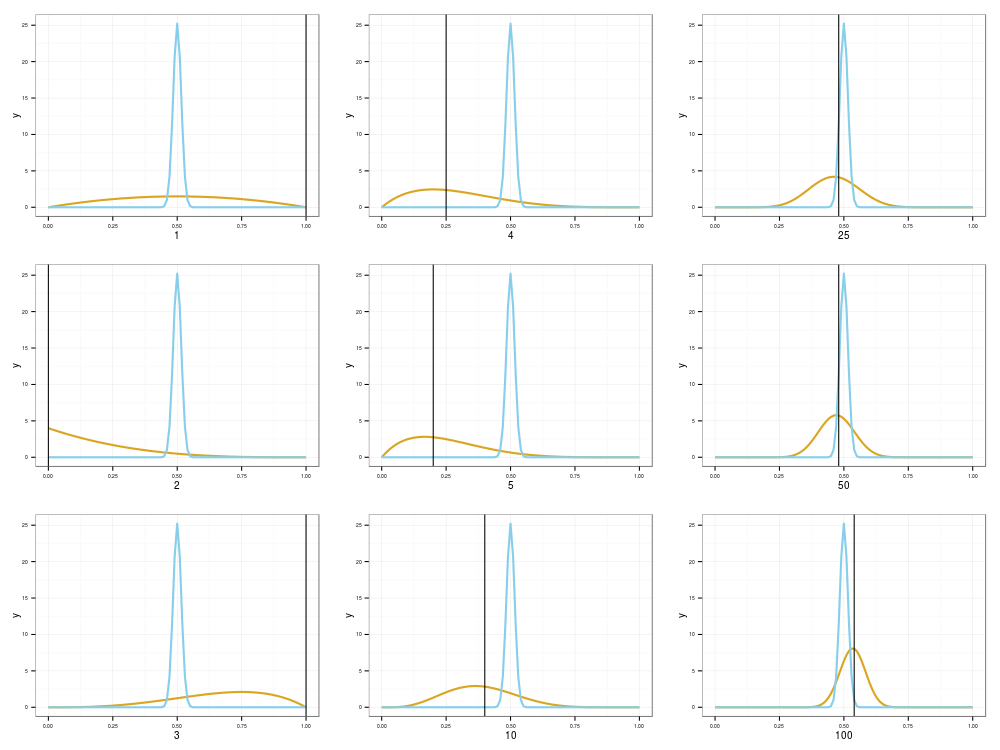
\includegraphics[height = \textheight,width=\textwidth,keepaspectratio=true]{figure/env_post_inspect}
  \caption{<+caption text+>}
  \label{fig:env_post}
\end{figure}

\begin{figure}[ht]
  \centering
  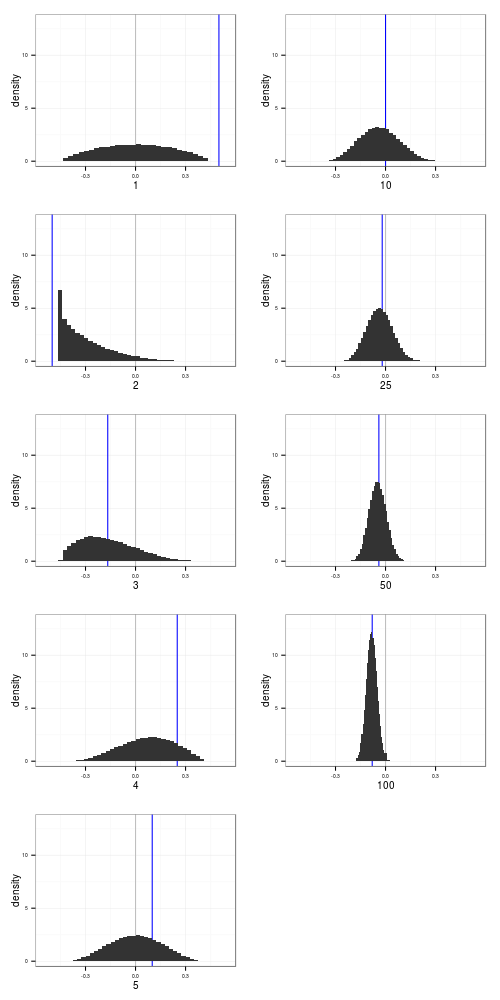
\includegraphics[height = \textheight,width=\textwidth,keepaspectratio=true]{figure/env_diff}
  \caption{<+caption text+>}
  \label{fig:env_diff}
\end{figure}

By defining environmental preference as the difference in full posterior estimates of occurrence probability, it is possible to include taxa with low sample sizes that are normal discarded \citep{Foote2006,Miller2001,Simpson2009,Kiessling2007a}. Additionally, 55+\% of observed Paleozoic brachiopod genera have less than 10 occurrences which is the sample size range where MAP (or ML) estimates would be most biased.
This is preferable to the difference in MAP estimates, especially for taxa with small sample sizes (blue line; Fig. \ref{fig:env_diff}).


% behavior of MAP estimates
%   as sample size increases, converge on true (10+)
% behavior of posterior
%   compromise between likelihood of data occurrences and (flat) prior
%   really important for small sample sizes
%   at 10+ makes no difference anymore
%   this is also kind obvious from the estimates of \(v\)
% how many taxa have less than 10 occurrences? \approx 55\%

\subsection{Survival model}

Genus durations were modeled in a Bayesian parameteric survival analysis framework. Durations were assumed to follow either an exponential or Weibull distribution. Each of these distributions makes strong assumptions about how duration may effect extinction risk. Use of the exponential distribution assumes that extinction risk is independent of duration. In contrast, use of the Weibull distribution allows for age dependent extinction via the shape parameter \(\alpha\), though only as a monotonic function of duration. Importantly, the Weibull distribution is equivalent to the exponential distribution when \(\alpha = 1\). In general, the notation used here follows \citet{Gelman2007}, \citet{Gelman2013d}, and \uppercase{stan manual}.

The simplest model of genus duration includes no covariate or structural information. Define \(y_{i}\) as the duration in stages of genus \(i\), where \(i = 1, \dots, n\) and \(n\) is the number of observed genera. These two models are them simply defined as
\begin{equation}
  \begin{aligned}
    y_{i} &\sim \mathrm{Exponential}(\lambda) \\
    y_{i} &\sim \mathrm{Weibull}(\alpha, \sigma).
  \end{aligned}
  \label{eq:simple}
\end{equation}
Note that \(\lambda\) is a ``rate'' or inverse-scale while \(\sigma\) is a scale parameter, meaning that \(\frac{1}{\lambda} = \sigma\).

These simple models can then be expanded to include covariate information as predictors by reparameterizing \(\lambda\) and \(\sigma\) as a regression \citep{Klein2003}. Each of the covariates of interest is given its own regression coefficient (e.g. \(\beta_{range}\)) along with an intercept term \(\beta_{0}\). There are some additional complications to the parameterization of \(\sigma\) associated with the inclusion of \(\alpha\) as well as interpretability \citep{Klein2003}. Both of these cases are written more fully as
\begin{equation}
  \begin{aligned}
    \lambda_{i} &= \exp(\beta_{0} + \beta_{r} r_{i} + \beta_{v} v_{i} + \beta_{v^{2}} v_{i}^{2} + \beta_{m} m_{i}) \\
    \sigma_{i} &= \exp\left(\frac{-(\beta_{0} + \beta_{r} r_{i} + \beta_{v} v_{i} + \beta_{v^{2}} v_{i}^{2} + \beta_{m} m_{i})}{\alpha}\right).
  \end{aligned}
  \label{eq:regression}
\end{equation}
The regression equations are exponentiated because both \(\lambda\) and \(\sigma\) are only defined for positive reals. The quadratic term for environmental affinity \(v\) is to allow for the possiblity of a nonlinear relationship between environmental affinity and extinction risk.

The models which incorporate both equations \ref{eq:simple} and \ref{eq:regression} can then be further expanded to allow all of the \(\beta\) coefficients, including \(\beta_{0}\), to vary with origination cohort while also modeling their covariance and correlation. This is called a varying-intercepts, varying-slopes model \citep{Gelman2007}. It is much easier to represent and explain how this is parameterized using matrix notation. First, define \(\mathbf{B}\) as \(k \times J\) matrix of the \(k\) coefficients including the intercept term (\(k = 5\)) for each of the \(J\) cohorts. Second, define \(\mathbf{X}\) as a \(n \times k\) matrix where each column is one of the covariates of interest. Importantly, \(\mathbf{X}\) includes a columns of all 1s which correspond to the constant term \(\beta_{0}\). Third, define \(j[i]\) as the origination cohort of genus \(i\), where \(j = 1, \dots, J\) and \(J\) is the total number of observed cohorts.

Using the above hierarchical expansion to the model, we then rewrite \(\lambda\) and \(\sigma\) in matrix notation as
\begin{equation}
  \begin{aligned}
    \lambda_{i} &= \exp(\mathbf{X}_{i} \mathbf{B}_{j[i]}) \\
    \sigma_{i} &= \exp\left(\frac{-(\mathbf{X}_{i} \mathbf{B}_{j[i]})}{\alpha}\right). 
  \end{aligned}
  \label{eq:multivariate}
\end{equation}

At face value, the above parameterization (Eq. \ref{eq:multivariate}) is opaque as to how the covariance and correlation between elements of \(\mathbf{B}\) are estimated. This becomes more apparent after defining the prior distribution of \(\mathbf{B}\). Because \(\mathbf{B}\) is a matrix, I used a multivariate normal prior with unknown vector of means \(\mu\) and covariance matrix \(\mathbf{\Sigma}\). This is written as 
\begin{equation}
  \mathbf{B} \sim \mathrm{MVN}(\mu_{\mathbf{B}}, \Sigma_{\mathbf{B}}).
  \label{eq:beta_prior}
\end{equation}
\(\mu_{\mathbf{B}}\) is length \(k\) vector representing the overall mean of the distributions of \(\beta\) coefficients. \(\Sigma_{\mathbf{B}}\) is a \(k \times k\) covariance matrix of the \(\beta\) coefficients.

What remains is assigning priors the elements of \(\mu_{\mathbf{B}}\) and the covariance matrix \(\Sigma_{\mathbf{B}}\). Each of the elements of vector \(\mu_{\mathbf{B}}\) were given independent, weakly-informative normal priors. The prior for \(\Sigma_{\mathbf{B}}\) is a bit more complicated. While the conjugate prior distribution for a covariance matrix is the inverse-Wishart \citep{Gelman2013d}, because I am using a variant for Hamiltonian Monte Carlo (HMC) called No U-Turn Sampling (NUTS) for posterior estimation as opposed to Gibbs sampling there is not benefit for using a conjugate prior \uppercase{stan manual}. Additionally, the inverse-Wishart distribution strongly constraints the off-diagonal elements of the covariance matrix. Instead, it is better to model the correlation matrix and separate variance terms for each of the \(k\) coefficients. This is possible because of the relationship between a covariance and a correlation matrix, defined as 
\begin{equation}
  \Sigma_{\mathbf{B}} = \text{Diag}(\tau_{B}) \Omega_{\mathbf{B}} \text{Diag}(\tau_{B})
  \label{eq:covcor}
\end{equation}
where \(\tau_{B}\) is a length \(k\) vector of variances and Diag(\(\tau_{B}\)) is a diagonal matrix.

I used a LKJ prior distribution for \(\Omega_{\mathbf{B}}\) as recommended by \uppercase{stan manual}. An LKJ is a single parameter multivariate distribution where values of \(\eta\) greater than 1 concentrate density at the unit correlation matrix, which corresponds to no correlation between the \(\beta\) coefficients. The scale parameter, \(\tau_{B}\), is given a weakly informative half-Cauchy (C\(^{+}\)) prior following \citet{Gelman2006a}.

Given all the above, the exponential distribution based model is then defined, including priors, as 
\begin{equation}
  \begin{aligned}
    y_{i} &\sim \mathrm{Exponential}(\lambda) \\
    \lambda_{i} &= \exp(\mathbf{X}_{i} \mathbf{B}_{j[i]}) \\
    \mathbf{B} &\sim \mathrm{MVN}(\mu_{\mathbf{B}}, \Sigma_{\mathbf{B}}) \\
    \Sigma_{\mathbf{B}} &= \text{Diag}(\tau_{B}) \Omega_{\mathbf{B}} \text{Diag}(\tau_{B}) \\
    \mu_{\kappa} &\sim \mathcal{N}(0, 5) \text{ for } \kappa \in 1:k \\
    \tau_{\kappa} &\sim \mathrm{C^{+}}(1) \text{ for } \kappa \in 1:k \\
    \Omega &\sim \text{LKJ}(2).
  \end{aligned}
  \label{eq:exp_total}
\end{equation}
The Weibull distribution based model is then also defined as
\begin{equation}
  \begin{aligned}
    y_{i} &\sim \mathrm{Weibull}(\alpha, \sigma) \\
    \sigma_{i} &= \exp\left(\frac{-(\mathbf{X}_{i} \mathbf{B}_{j[i]})}{\alpha}\right) \\
    \mathbf{B} &\sim \mathrm{MVN}(\mu_{\mathbf{B}}, \Sigma_{\mathbf{B}}) \\
    \Sigma_{\mathbf{B}} &= \text{Diag}(\tau_{B}) \Omega_{\mathbf{B}} \text{Diag}(\tau_{B}) \\
    \alpha &\sim \mathrm{C^{+}}(2) \\
    \mu_{\kappa} &\sim \mathcal{N}(0, 5) \text{ for } \kappa \in 1:k \\
    \tau_{\kappa} &\sim \mathrm{C^{+}}(1) \text{ for } \kappa \in 1:k \\
    \Omega &\sim \text{LKJ}(2).
  \end{aligned}
  \label{eq:wei_total}
\end{equation}
Note that the above formulations of each model (Eq. \ref{eq:exp_total}, \ref{eq:wei_total}) does not include how the uncertainty in environmental affinity is included nor how censored observations are included. An explination of including censored observations follows.


\subsection{Censored observations}
A key aspect of survival analysis is the inclusion of censored, or incompletely observed, data points \citep{Ibrahim2001,Klein2003}. The two classes of censored observations encountered in this study were right and left censored observations. Right censored genera are those that did not go extinct during the window of observation, or genera that are still extant. Left censored observations are those taxa that it is only known when it was extinct by. To put another way, this is a taxon that went extinct but the observed duration is an over estimate of the actual duration. 

In the context of this study, I considered all genera that had a duration of only one geologic stage to be left censored as we do not have a finer degree of resolution. Conceptually, this is similar to if I was studying, say, survival patterns in rats and an individual had died between the start of the experiment and next time the rats were observed. We know the rat lived no more than day.

The key function for modeling censored observations is the survival function, or \(S(t)\). \(S(t)\) corresponds to the probability that a genus having existed for \(t\) stages will not have gone extinct while \(h(t)\) corresponds to the instantaneous extinction rate at taxon age \(t\) \cite{Klein2003}. For an exponential model, \(S(t)\) is defined as
\begin{equation}
  S(t) = \exp(-\lambda t),
  \label{eq:exp_surv}
\end{equation}
and for the Weibull distribution \(S(t)\) is defined as
\begin{equation}
  S(t) = \exp\left(-\left(\frac{t}{\sigma}\right)^{\alpha}\right).
  \label{eq:wei_surv}
\end{equation}
\(S(t)\) is equivalent to the complementary cumulative distribution function, \(1 - F(t)\) \citep{Klein2003}. 

For right censored observations, instead of calculating the likelihood as normal (Eq. \ref{eq:multivariate}) the likelihood of an observation is evaluated using \(S(t)\). Conceptually, this approach calculates the likelihood of observing a taxon that existed for at least that long. For left censored data, instead the likelihood is calculated using \(1 - S(t)\) which corresponds to the likelihood of observing a taxon that existed no longer than \(t\).

The full likelihood statements incorporating fully observed, right censored, and left censored observations are then
\begin{equation}
  \begin{aligned}
    \mathcal{L} &\propto \prod_{i \in C} \mathrm{Exponential}(y_{i} | \lambda) \prod_{j \in R} S(y_{j} | \lambda) \prod_{k \in L} \left(1 - S(y_{k} | \lambda)\right) \\
    \mathcal{L} &\propto \prod_{i \in C} \mathrm{Weibull}(y_{i} | \alpha, \sigma) \prod_{j \in R} S(y_{j} | \alpha, \sigma) \prod_{k \in L} \left(1 - S(y_{k} | \alpha, \sigma)\right)
  \end{aligned}
  \label{eq:censored_likelihood}
\end{equation}
where \(C\) is the set of all fully observed taxa, \(R\) the set of all right censored taxa, and \(L\) the set of all left-censored taxa.


\subsection{Parameter estimation}
Given the above likelihood and prior statements, the posterior probabilities of all parameters was approximated using a Markov-chain Monte Carlo routine using a variant of Hamiltonian Monte Carlo called the No-U-Turn Sampler \citep{Hoffman2014} as implemented in the probabilistic programming language Stan \citep{stan-software:2014}. The estimate of the posterior distribution were approximated from four parallel chains run for 10000 draws split half warm-up and half sampling thinned to every 10 sample for a total of 5000 samples. Chain convergence was assessed via the scale reduction factor \(\hat{R}\) where values close to 1 (\(\hat{R} < 1.1\)) indicate approximate convergence. Convergence means that the chains are approximately stationary and the samples are well mixed \citep{Gelman2013d}.


\subsection{Model evaluation}

Models were evaluated using both a series of multiple posterior predictive checks and an estimate of out-of-sample predictive accuracy. 

The motivation behind posterior predictive checks as tools for determining model adequacy is that replicated data sets using the fitted model should be similar to the original data \citep{Gelman2013d}. Systematic differences between the simulations and observed indicate weaknesses of the currently fit model. An example of a technique that is very similar would be inspecting the residuals and Q-Q plots from a linear regression.

The strategy behind posterior predictive checks is to draw simulated values from the joint posterior predictive distribution, \(p(y^{rep} | y)\), and then compared to the original observed values \citep{Gelman2013d}. To accomplish this, for each replicate, a single value is drawn from the marginal posterior distributions of each regression coefficient from the final model (Eq. \ref{eq:exp_total}, \ref{eq:wei_total}). Then, given the covariate information for each of the observations \(\mathbf{X}\), a new set of \(n\) genus durations are generated giving a single replicated data set \(y^{rep}\). This is repeated 1000 times in order to provide a distribution of possible values that could have been observed given the model. 

In order to compare the fitted model to the observed data, various graphical comparisons or test quantities need to be defined. The principal comparison used here is a comparison between non-parameteric approximation of the survival function \(S(t)\) as estimated from both the observed data and each of the replicated data sets. The purpose of this comparison is to determine if the model approximates the same survival/extinction pattern as the original data. 

I also did a graphical examination of the deviance residuals. While normal residuals are defined as \(y_{i}^{rep} - y_{i}\), deviance residuals are a specific class of residuals derived with non-normal errors in mind. The definition of deviance residuals for a Weibull regression, of which the above models can be considered, is as follows. First define the cumulative hazard function \(\Lambda(t)\) for the Weibull distribution \citep{Klein2003}. Given \(S(t)\) (Eq. \ref{eq:wei_surv}), the cumulative hazard function is 
\begin{equation}
  \Lambda(t) = -log\left(S\left(t\right)\right).
\end{equation}

Next, define martingale residuals \(m\) as
\begin{equation}
  m_{i} = I_{i} - \Lambda(t_i).
\end{equation}
\(I\), called the inclusion vector, is vector of length \(n\) where \(I_{i} = 1\) means the observation is completely observed and \(I_{i} = 0\) means the observation is censored. Martingale residuals have a mean of 0, range between 1 and \(-\infty\), and can be viewed as the difference between the observed number of deaths between 0 and \(t_{i}\) and the expected number of deaths based on the model. However, martingale residuals are asymmetrically distributed, and can not be interpreted in the same manner as standard residuals. 

The solution to this is to use deviance residuals, \(D\), which are defined as a function of martingale residuals and takes the form
\begin{equation}
  D_{i} = \text{sign}(m_{i}) \sqrt{-2[m_{i} + I_{i}log(I_{i} - m_{i})]}.
\end{equation}
Deviance residuals have a mean of 0 and a standard deviation of 1 by definition \citep{Klein2003}.

The exponential and Weibull models were compared for out-of-sample predictive accuracy using the widely-applicable information criterion (WAIC) \citep{Watanabe2010a}. Because the Weibull model reduces to the exponential model when \(\alpha = 0\), our interest is not in choosing between these models. Instead comparison of WAIC values is useful for better understanding the effect of model complexity on out-of-sample predictive accuracy. The calculation of WAIC used here corresponds to the ``WAIC 2'' formulation recommended by \citet{Gelman2013d}.

WAIC can be considered fully Bayesian alternative to the Akaike information criterion, where WAIC acts as an approximation of leave-one-out cross-validation which acts as a measure of out-of-sample predictive accuracy. WAIC is calculated starting with the log pointwise posterior predictive density calculated as
\begin{equation}
  \mathrm{lppd} = \sum_{i = 1}^{n} \log \left(\frac{1}{S} \sum_{s = 1}^{S} p(y_{i}|\Theta^{S})\right),
  \label{eq:lppd}
\end{equation}
where \(n\) is sample size, \(S\) is the number posterior simulation draws, and \(\Theta\) represents all of the estimated parameters of the model. This is similar to calculating the likelihood of each observation given the entire posterior. A correction for the effective number of parameters is then added to lppd to adjust for overfitting. The effective number of parameters is calculated, following derivation and recommendations of \citep{Gelman2013d}, as
\begin{equation}
  p_{\mathrm{WAIC}} = \sum_{i = 1}^{n} V_{s = 1}^{S} (\log p(y_{i}|\Theta^{S})).
  \label{eq:pwaic}
\end{equation}
where \(V\) is the sample posterior variance of the log predictive density for each data point.

Given both equations \ref{eq:lppd} and \ref{eq:pwaic}, WAIC is then calculated
\begin{equation}
  \mathrm{WAIC} = \mathrm{lppd} - p_{\mathrm{WAIC}}.
  \label{eq:waic}
\end{equation}
When comparing two or more models, lower WAIC values indicate better out-of-sample predictive accuracy. Importantly, WAIC is just one way of comparing models. When combined with posterior predictive checks it is possible to get a more complete understanding of model fit.


\end{document}


\documentclass[12pt,letterpaper]{article}

\usepackage{amsmath, amsthm}
\usepackage{microtype, parskip}
\usepackage[comma,numbers,sort&compress]{natbib}
\usepackage{lineno}
\usepackage{docmute}
\usepackage{caption, subcaption, multirow, morefloats, rotating}
\usepackage{wrapfig}

\frenchspacing

\captionsetup[subfigure]{position = top, labelfont = bf, textfont = normalfont, singlelinecheck = off, justification = raggedright}

\begin{document}
\section{Results}

% Model fit
%   survival curve
%   deviance residuals
%   posterior predictive point tests
%   weibull > exponential (supported by WAIC)
As stated above, posterior approximations for both the exponential and Weibull models achieved approximate stationarity after 10,000 steps, as all parameter estimates have an \(\hat{R} < 1.1\).%\uppercase{ref tables}.

Comparisons of the survival functions estimated from 1000 posterior predictive data sets to the estimated survival function of the observed genera demonstrates that both the exponential and Weibull models approximately capture the observed pattern of extinction (Fig. \ref{fig:surv}). The major difference in fit between the two models is that the Weibull model has a slightly better fit for longer lived taxa than the exponential model.

\begin{figure}[ht]
  \centering
  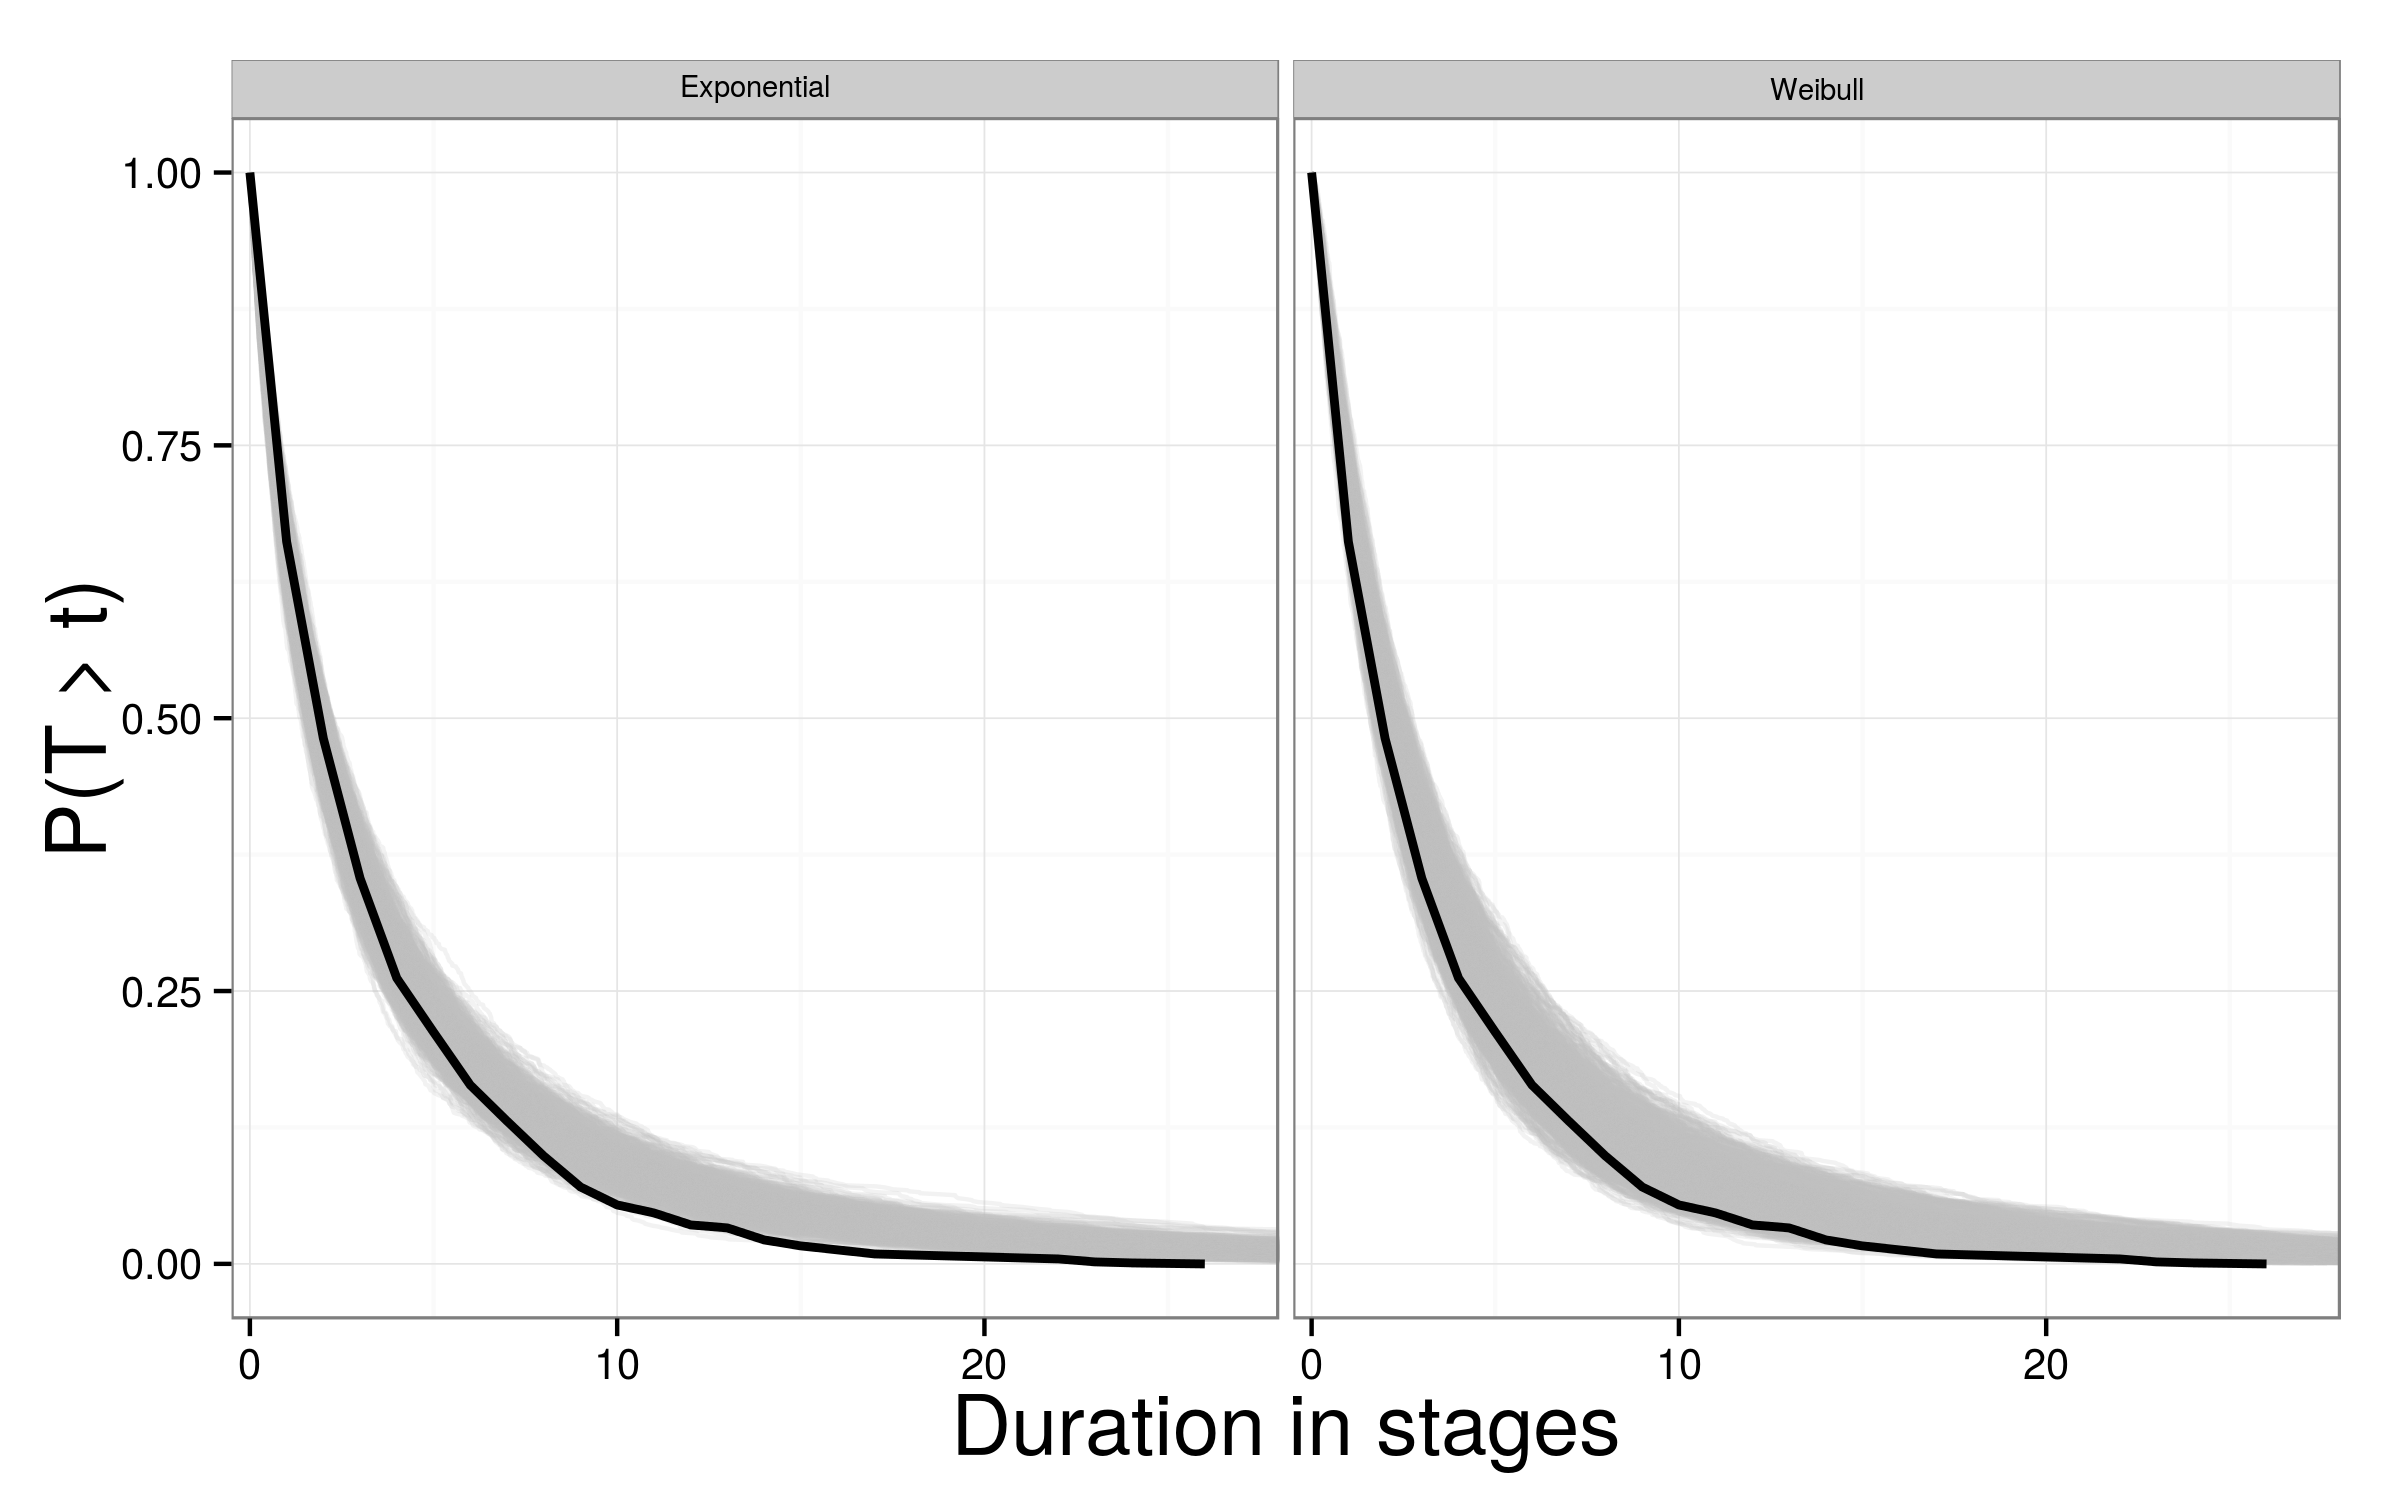
\includegraphics[height = 0.5\textheight,width=\textwidth,keepaspectratio=true]{figure/survival_curves}
  \caption{Comparison of empirical estimates of \(S(t)\) versus estimates from 1000 posterior predictive data sets. \(S(t)\) corresponds to \(P(T > t)\) as it is the probability that a given genus observed at age \(t\) will continue to live. This is equivalent to the probability that \(t\) is less than the genus' ultimate duration \(T\). Note that the Weibull (left) model has noticeably better fir to the data than the exponential (right).}
  \label{fig:surv}
\end{figure}

%Inspection of the deviance residuals yields a similar pattern of biased estimates for longer lived taxa \uppercase{ref figure}. 

Additionally, the Weibull model is expected to have slightly better out-of-sample predictive accuracy when compared to the exponential model \uppercase{values}. This is congruent with graphical comparisons of the survival functions (Fig. \ref{fig:surv}). Because the difference between the WAIC scores is small, both results from the exponential and Weibull models will be analyzed.

% Results/hypothesis tests
%   \mu of hierarchical effects
%   \tau of hierarchical effects (partial pooling)
Estimates of the overall overall mean covariate effects \(\mu\) can be considered time-invariant generalizations for brachiopod survival during the Paleozoic \uppercase{Smits in prep} (Fig. \ref{fig:mu}). Consistent with prior expectations, geographic range size has a negative effect on extinction risk where genera with large ranges having greater durations than genera with small ranges. I also find no time-invariant effect of body size on genus duration. 
\begin{figure}[ht]
  \centering
  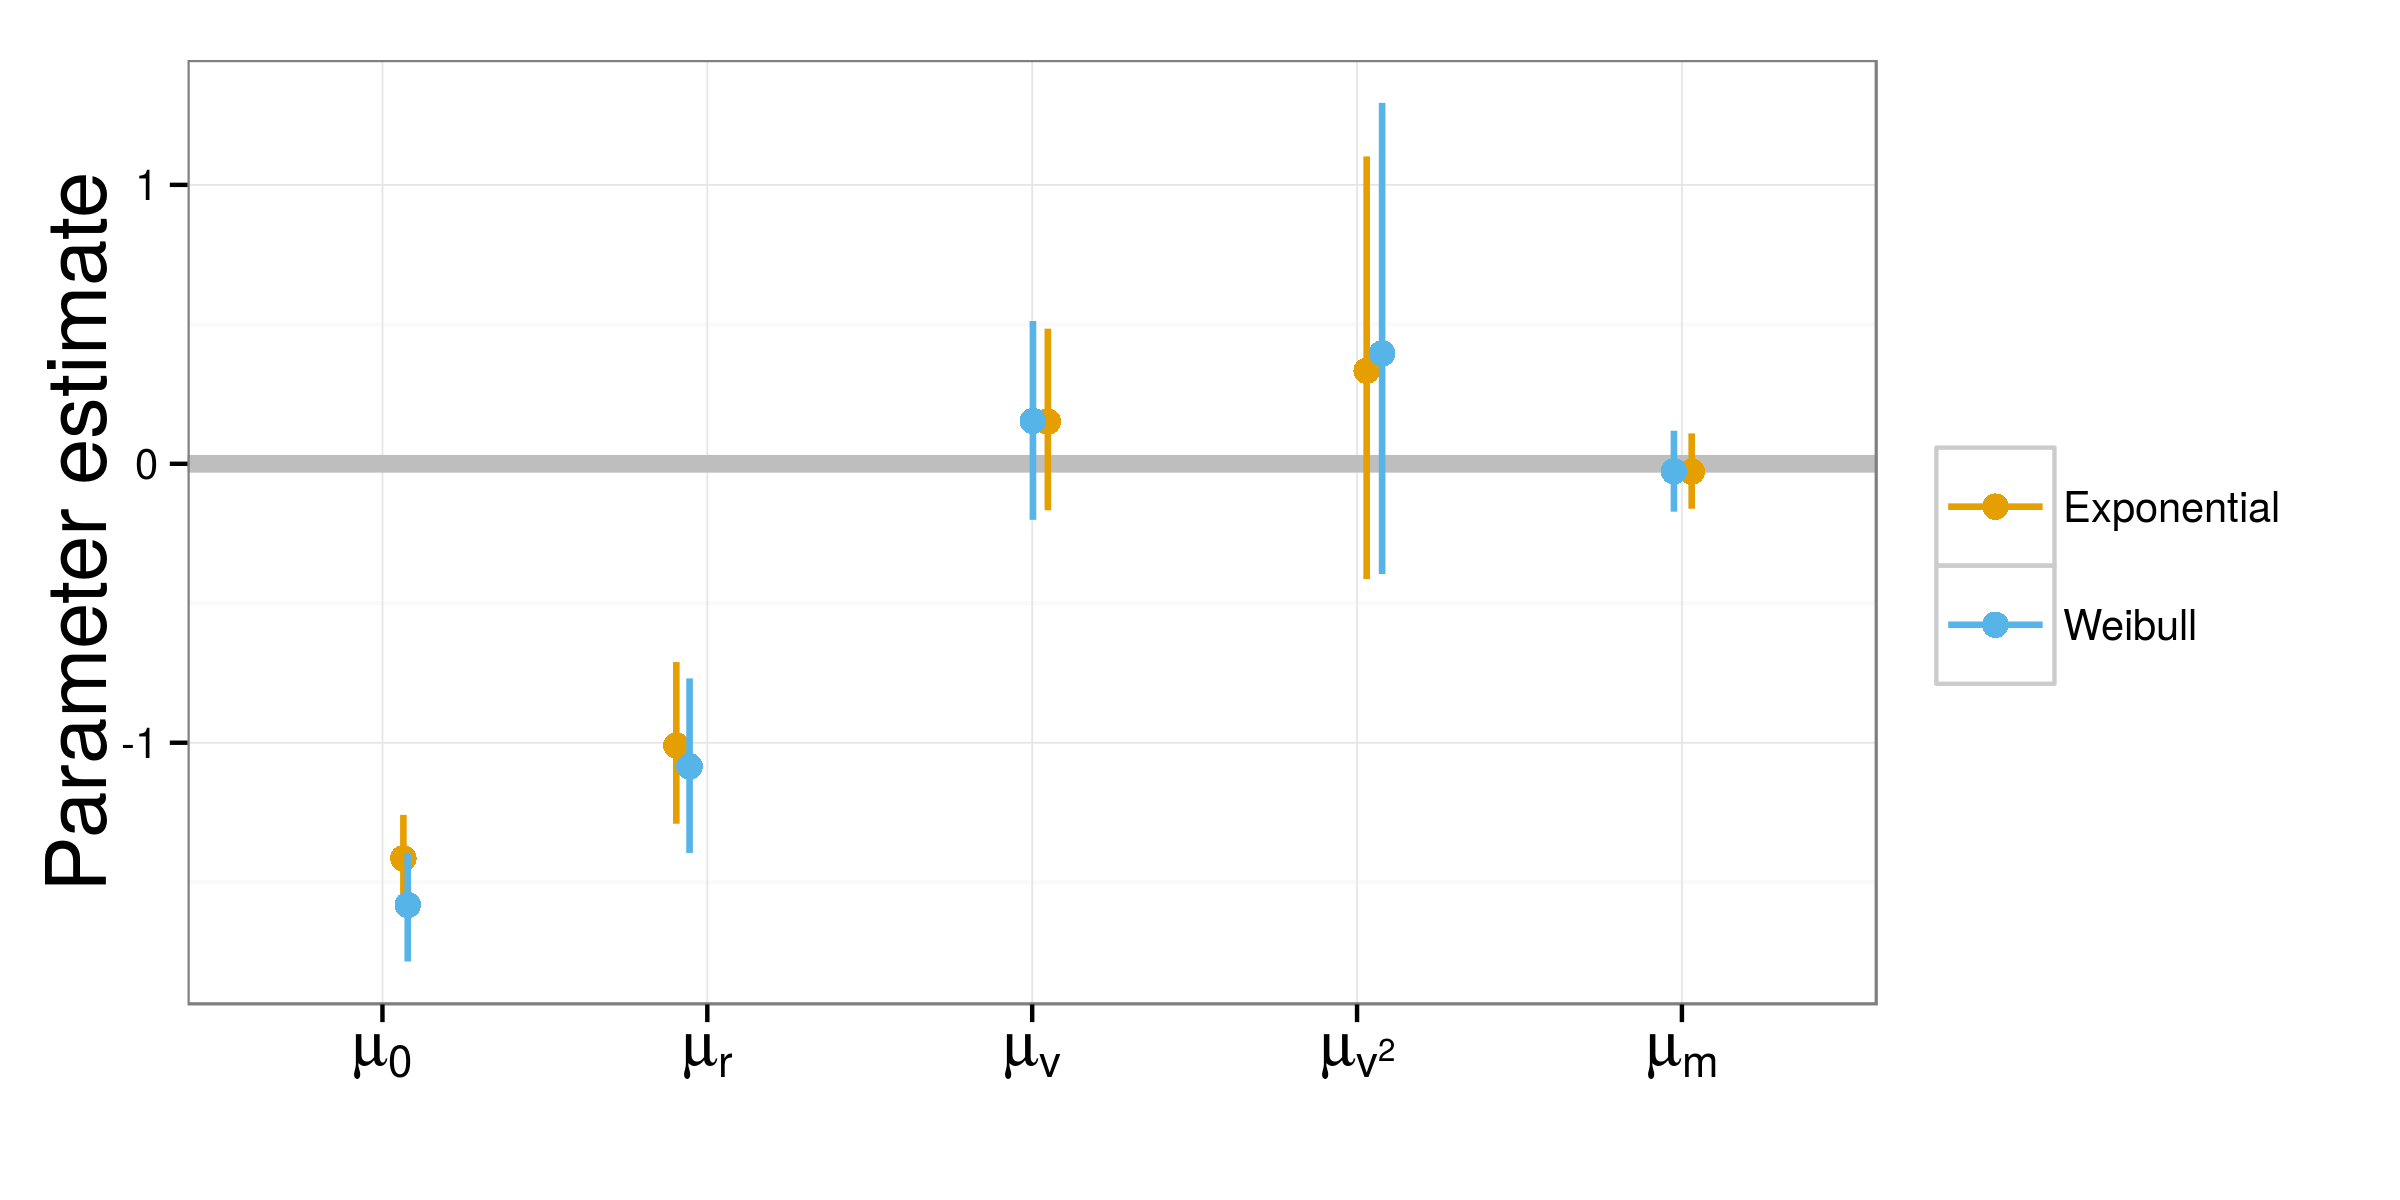
\includegraphics[height = 0.5\textheight,width=\textwidth,keepaspectratio=true]{figure/coef_means}
  \caption{<+caption text+>}
  \label{fig:mu}
\end{figure}

Interpretation of the effect of environmental preference \(v\) on duration is slightly more involved. Because a quadratic term is the equivalent of an interaction term, both \(\mu_{v}\) and \(\mu_{v^{2}}\) have to be interpreted together because it is illogical to change values of \(v\) without also changing values \(v^{2}\). To determine the nature of the effect of \(v\) on duration I calculated the multiplicative effect of environmental preference on extinction risk.

Given mean estimated extinction risk \(\tilde{\sigma}\), we can define the extinction risk multiplier of an observation with environmental preference \(v_{i}\) as 
\begin{equation}
  \frac{\tilde{\sigma_{i}}}{\tilde{\sigma}} = f(v_{i}) = \exp\left(\frac{-(\mu_{v} v_{i} + \mu_{v^{2}} v^{2})}{\alpha}\right).
  \label{eq:env}
\end{equation}
This exponentiated quadratic function \(f(v_{i})\) has a y-intercept of \(\exp(0)\) or 1 by definition as it does not have a specified non-zero intercept term. Equation \ref{eq:env} can be either upward or downward facing. A downward facing \(f(v_{i})\) indicates that genera of intermediate environmental preference have greater durations than either extreme, and \textit{vice versa} for upward facing functions.

The expected effect of environmental preference as a multiplier of expected extinction risk can then be visualized (Fig. \ref{fig:env_mean}). This figure depicts 1000 posterior predictive estimates of Eq. \ref{eq:env} across all possible values of \(v\). The number indicates the posterior probability that the function is downward facing, with generalists having lower extinction risk/greater duration than either type of specialist. Note that the inflection point/optimum of Fig. \ref{fig:env_mean} is approximately \(x = 0\), something that is expected given the estimate of \(\mu_{v}\) (Fig. \ref{fig:mu}).
\begin{figure}[ht]
  \centering
  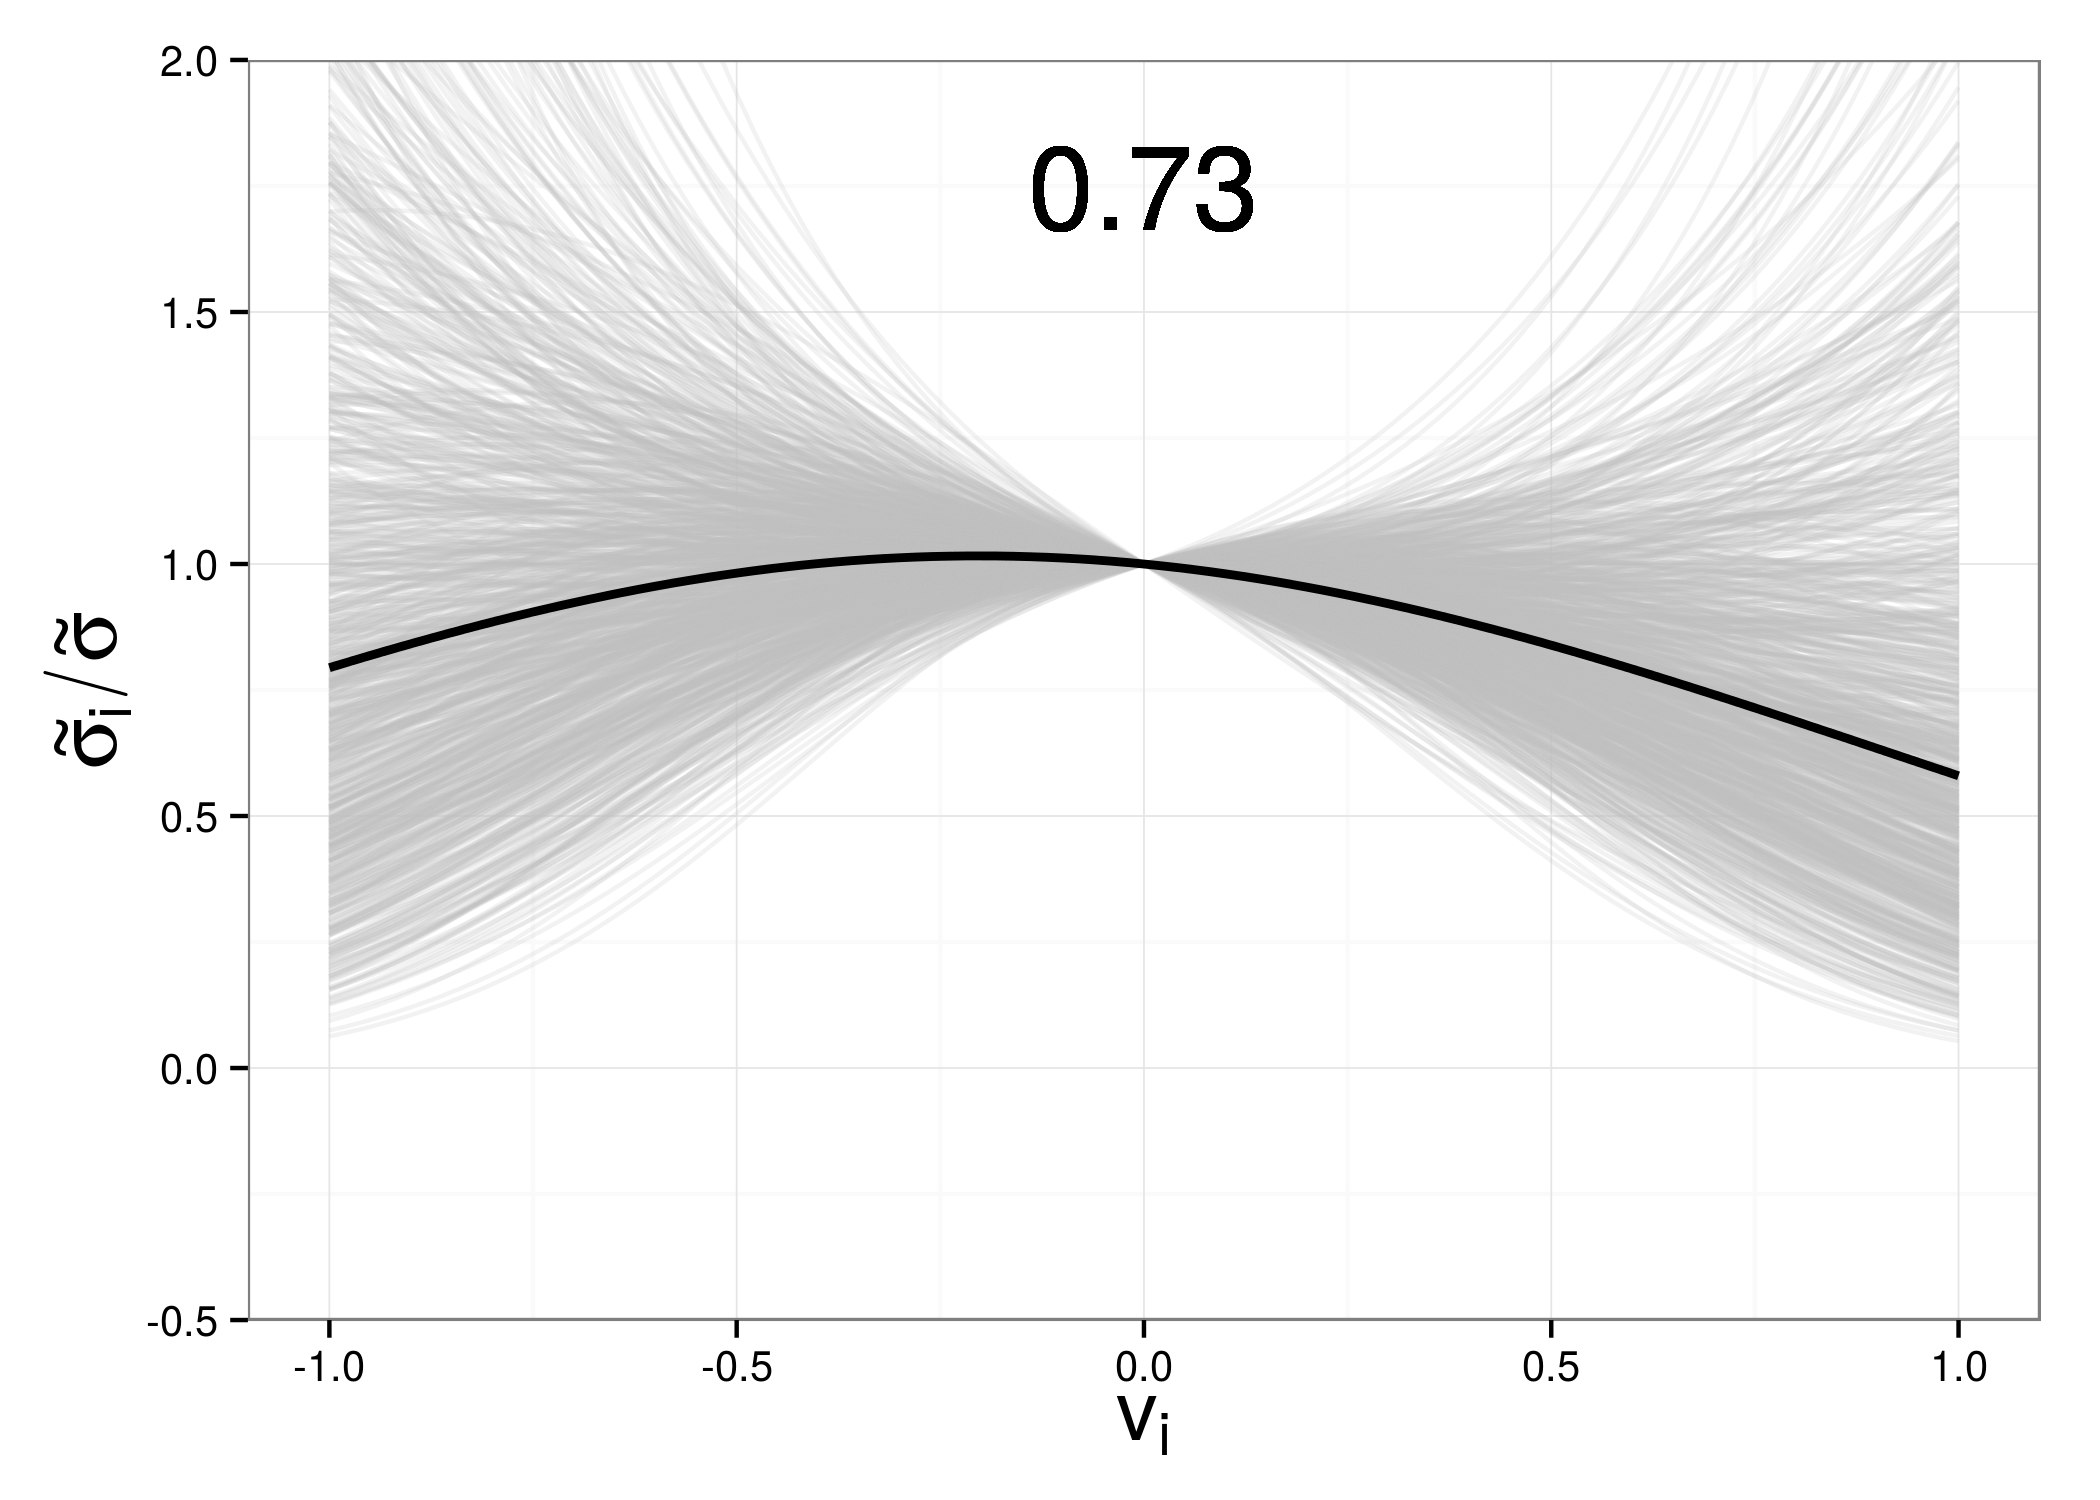
\includegraphics[height = 0.5\textheight,width=\textwidth,keepaspectratio=true]{figure/environ_quad}
  \caption{<+caption text+>}
  \label{fig:env_mean}
\end{figure}

The matrix \(\Sigma\) describing the covariance between the different coefficients describes how these coefficients might vary together across the origination cohorts. Similar to how this was modeled (Eq. \ref{eq:exp_total}, \ref{eq:wei_total}), for interpretation purposes \(\Sigma\) can be decomposed into a vector of standard deviations \(\vec{\tau}\) and a correlation matrix \(\Omega\).

The estimates of the standard deviation of between cohort coefficient estimates \(\tau\) vary greatly (Fig. \ref{fig:tau}). Coefficients with greater values of \(\tau\) have greater between cohort variation. The individual covariate effects with the greatest between origination cohort variation are \(\beta_{r}\), \(\beta_{v}\), and \(\beta_{v^{2}}\). \(\beta_{m}\) has negligible between cohort variation, as it has less have less between cohort variation than the between cohort variation in baseline extinction risk \(\beta_{0}\). However the amount between cohort variation in estimates of \(\beta_{v^{2}}\) mean that it is possible for the function describing the effect of environmental affinity can be upward facing for some cohorts (Eq. \ref{eq:env}), which corresponds to environmental generalists being shorted lived than specialists in that cohort.
\begin{figure}[ht]
  \centering
  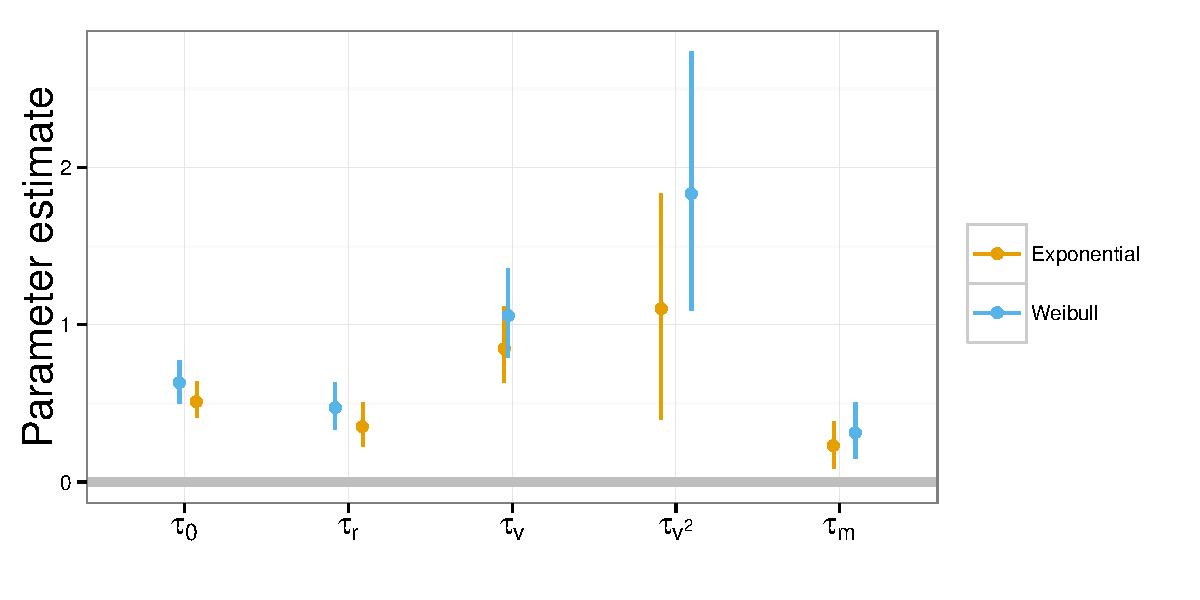
\includegraphics[height = 0.5\textheight,width=\textwidth,keepaspectratio=true]{figure/coef_var}
  \caption{<+caption text+>}
  \label{fig:tau}
\end{figure}


% omega heatmap
%   correlations with baseline extinction risk of of major interest
%   high/positive values of intercept --> high extinction risk
%   low/negative values of intercept --> low extinction risk
The correlation terms of \(\Omega\) (Fig. \ref{fig:omega}) describe the relationship between the coefficients and how their estimates may vary together across cohorts. The correlations between the intercept term \(\beta_{0}\) and the effects of the taxon traits are of particular interest for evaluating the \citet{Jablonski1986} hypothesis (Fig. \ref{fig:omega} first column/last row). Keep in mind that when \(\beta_{0}\) is low, extinction risk is low; and conversely, when \(\beta_{0}\) is high, then extinction risk is high.
\begin{figure}[ht]
  \centering
  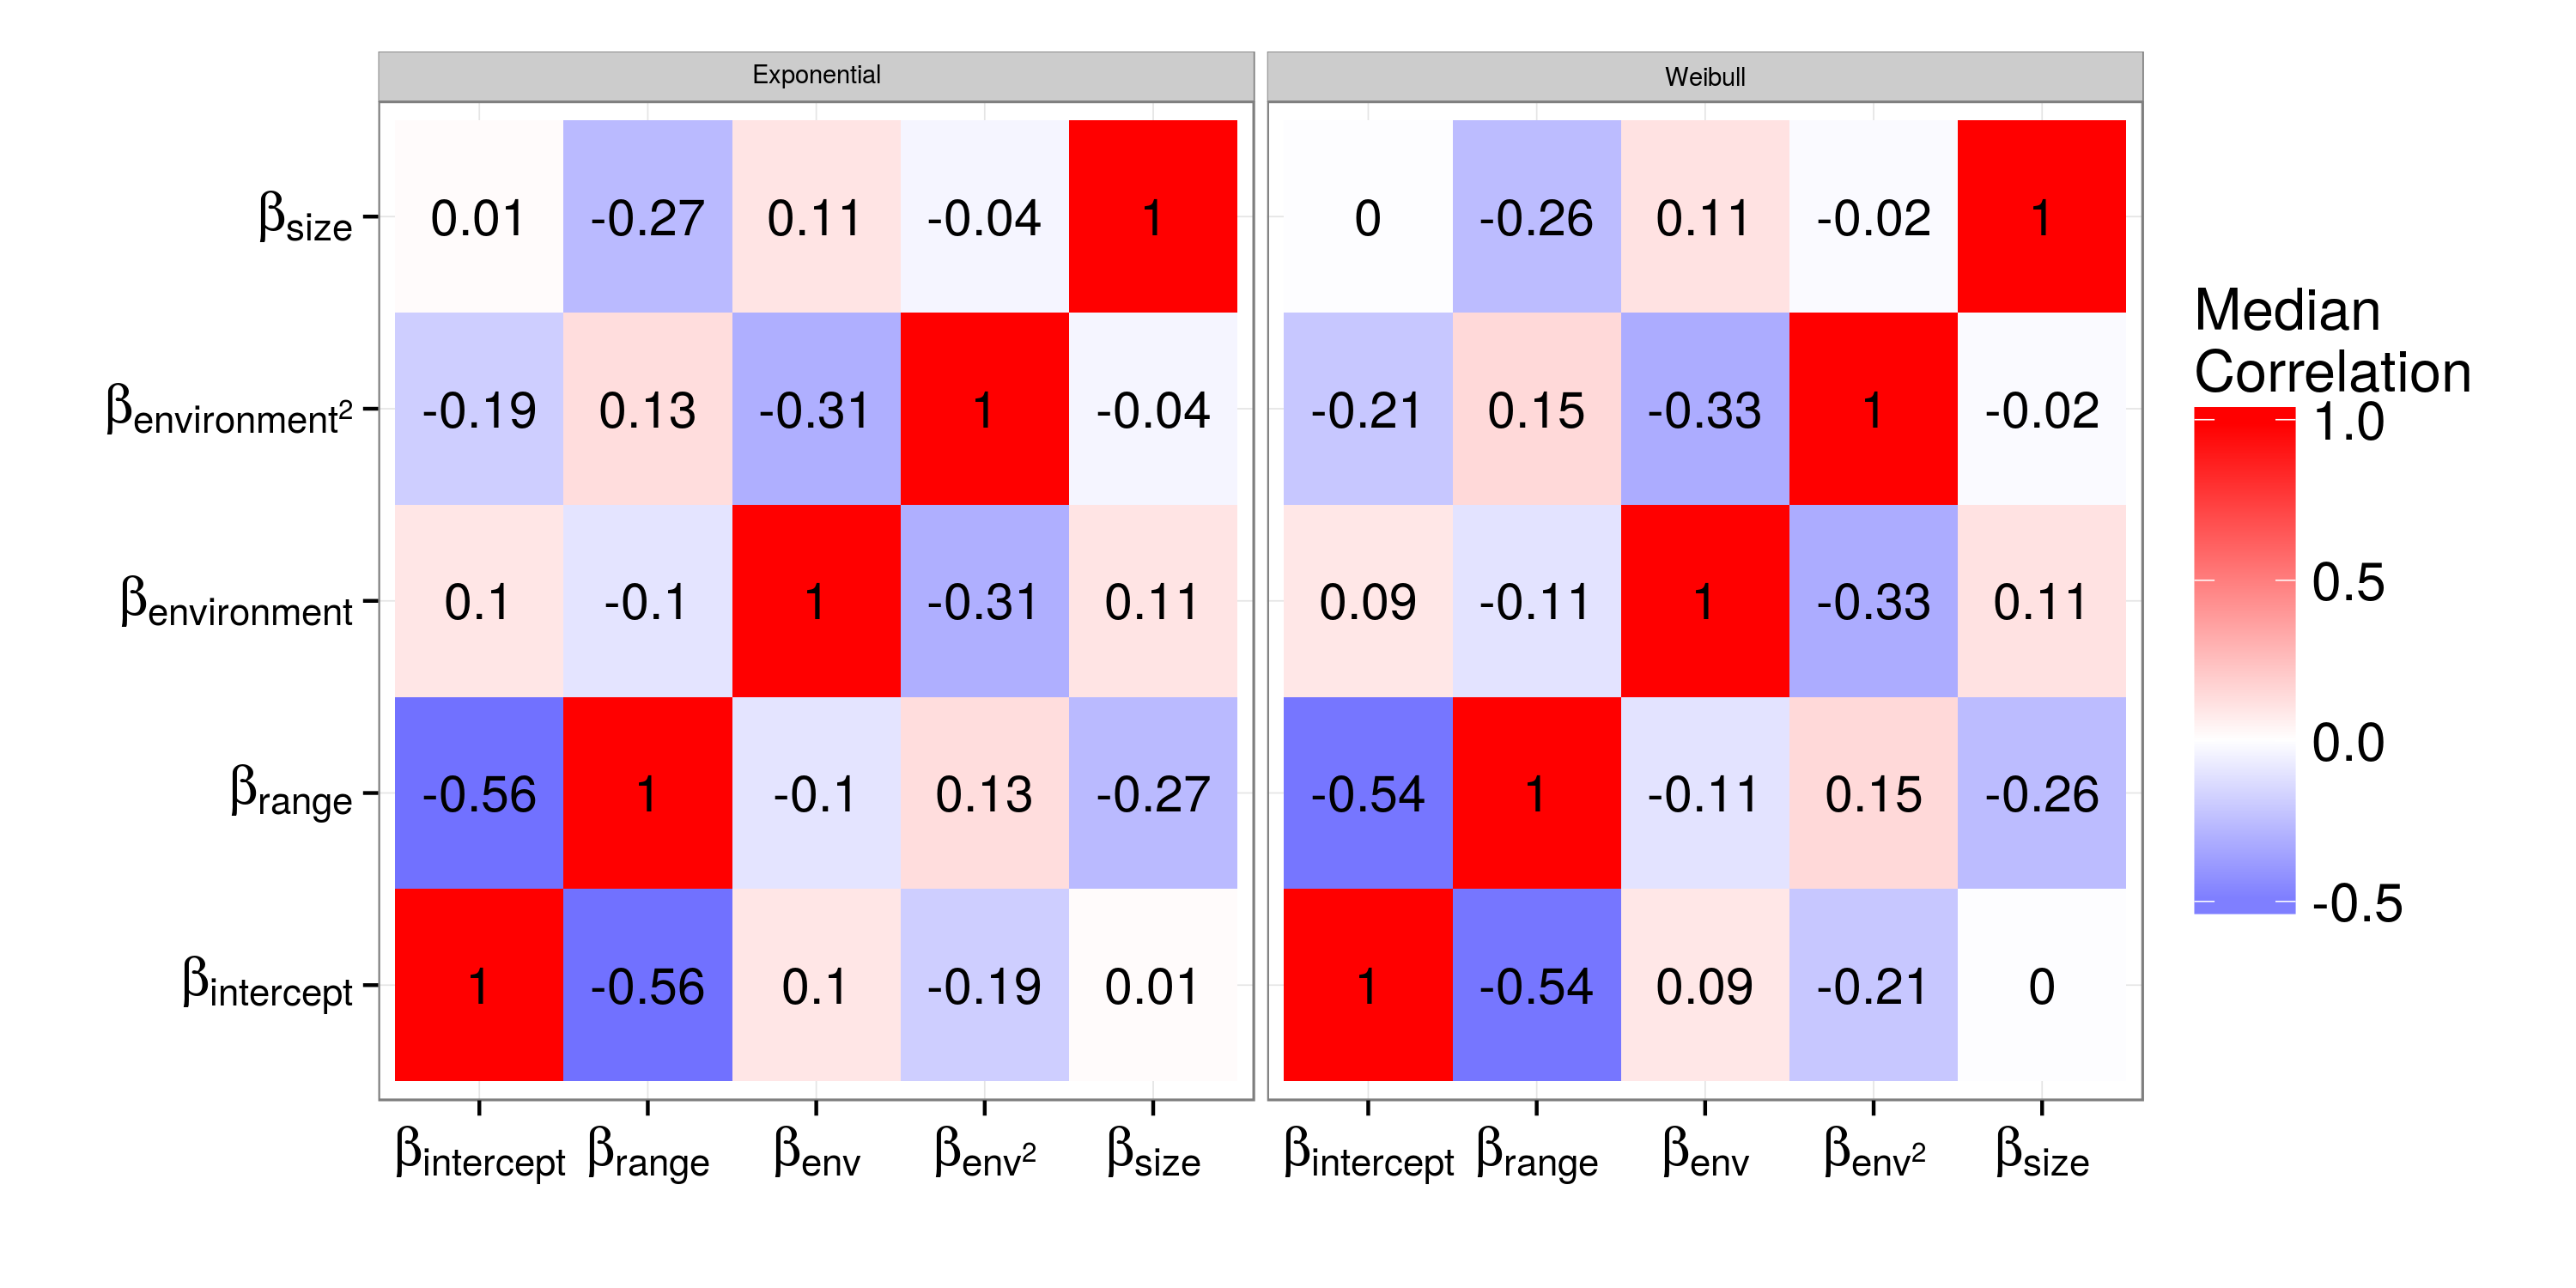
\includegraphics[height = 0.5\textheight,width=\textwidth,keepaspectratio=true]{figure/correlation_heatmap}
  \caption{<+caption text+>}
  \label{fig:omega}
\end{figure}

Marginal posterior probabilities of the correlation terms between the level of baseline extinction risk \(\beta_{0}\) and the effects of the taxon traits indicate that the correlation between between expected extinction risk and geographic range \(\beta_{r}\) is of particular note (Fig. \ref{fig:corr}). The negative correlation between \(\beta_{0}\) and \(\beta_{r}\) implies that as extinction risk increases, the effect/importance of geographic range on genus duration increases. This translates to mean that increases in baseline extinction rate are correlated with an increased importance of geographic range size. % this actually means that the effects of the other traits aren't going down, but instead aren't correlated with intensity and geographic range just gets more important!
\begin{figure}[ht]
  \centering
  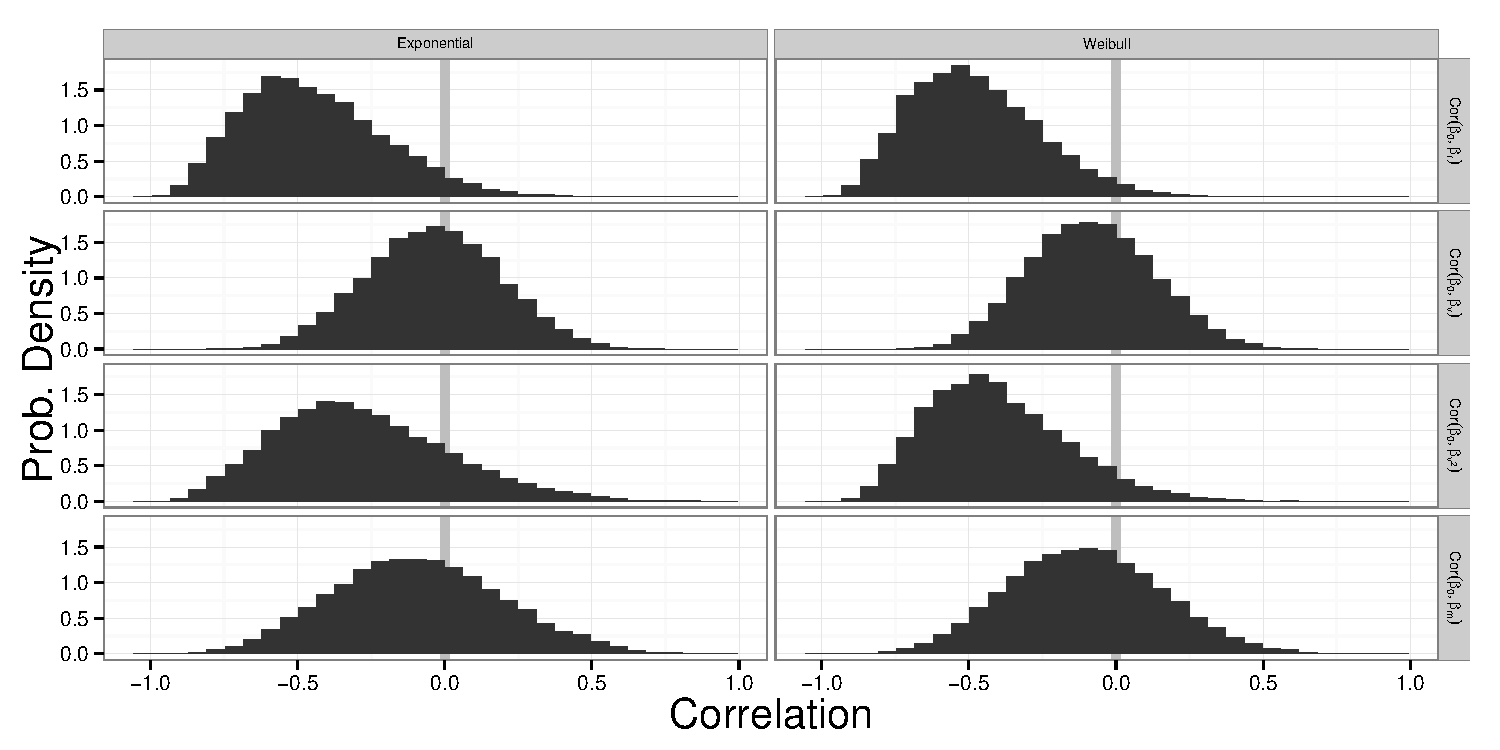
\includegraphics[height = 0.5\textheight,width=\textwidth,keepaspectratio=true]{figure/correlation_marginal}
  \caption{<+caption text+>}
  \label{fig:corr}
\end{figure}

% effects varying between cohorts
While the overall group level estimates are of particular importance when defining time-invariant differences in extinction risk, it is also important and useful to analyze the individual level parameter estimates in order to better understand how parameters actually vary across cohorts.

In comparison to the overall mean extinction risk \(\mu_{intercept}\), cohort level estimates \(\beta_{0}\) show some amount of variation through time as expected by estimates of \(\tau_{intercept}\) (Fig. \ref{fig:cohort_intercept}). A similar, if slightly greater, amount of variation is also observable in cohort estimates of the effect of geographic range \(\beta_{r}\) (Fig. \ref{fig:cohort_range}). Again, smaller values of \(\beta_{0}\) correspond to lower expected extinction risk. Similarly, smaller values of \(\beta_{r}\) correspond to greater decrease in extinction risk with increasing geographic range 
\begin{figure}[ht]
  \centering
  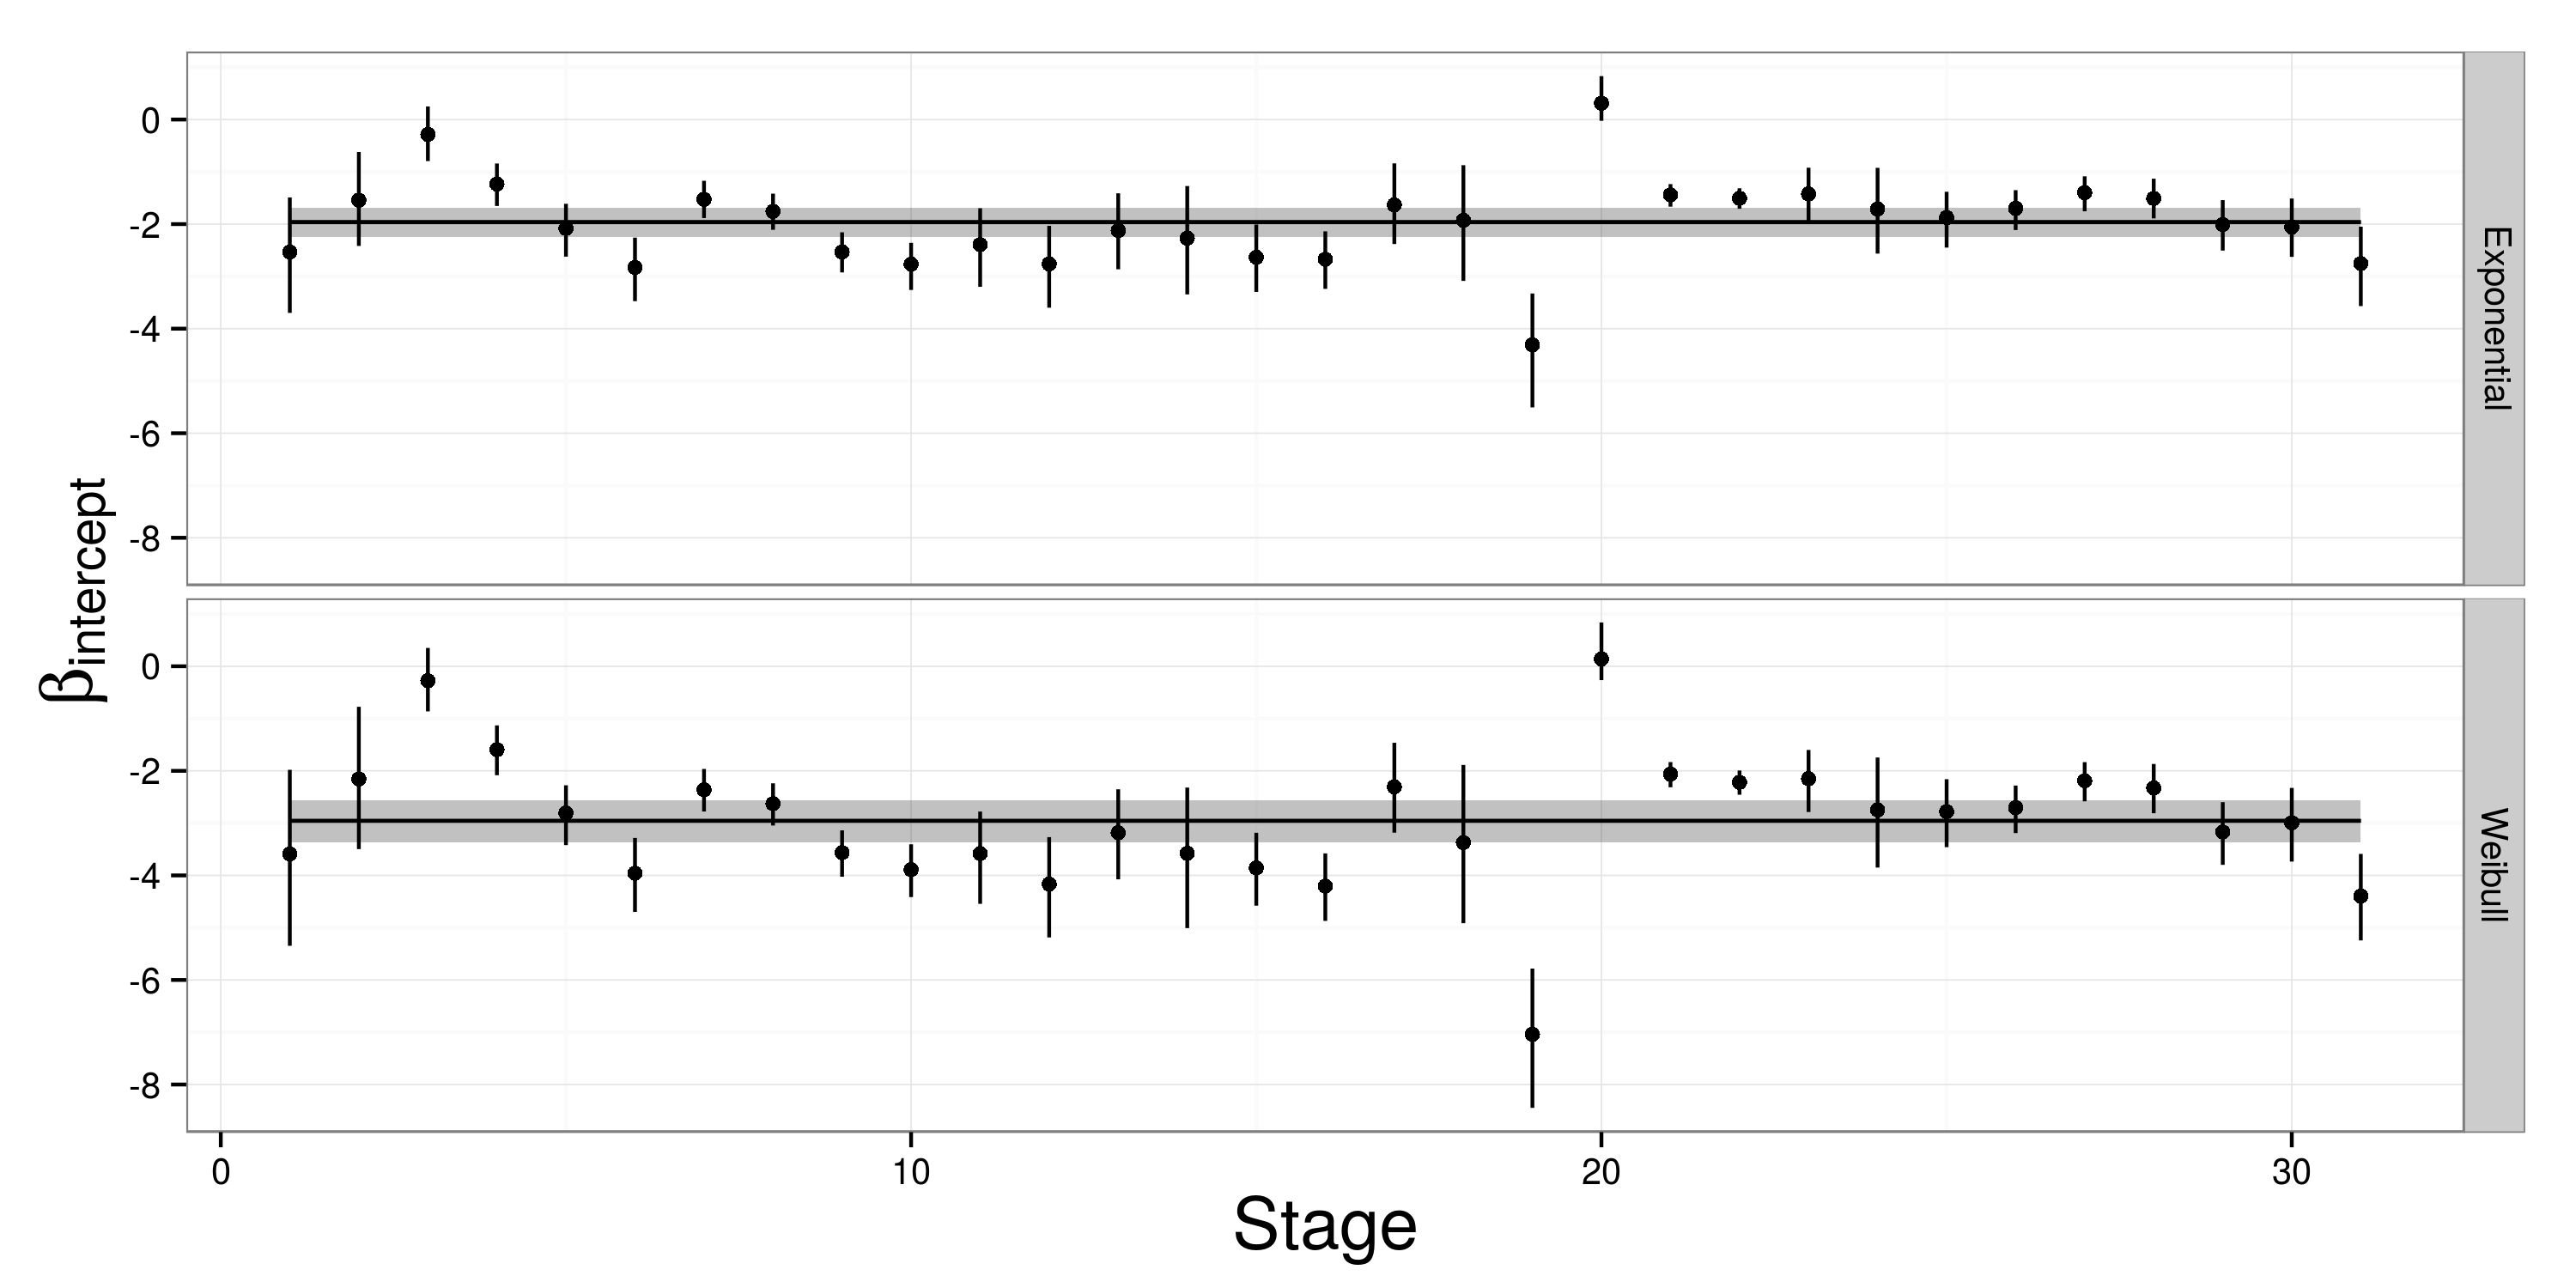
\includegraphics[height = 0.5\textheight,width=\textwidth,keepaspectratio=true]{figure/intercept_cohort}
  \caption{<+caption text+>}
  \label{fig:cohort_intercept}
\end{figure}

\begin{figure}[ht]
  \centering
  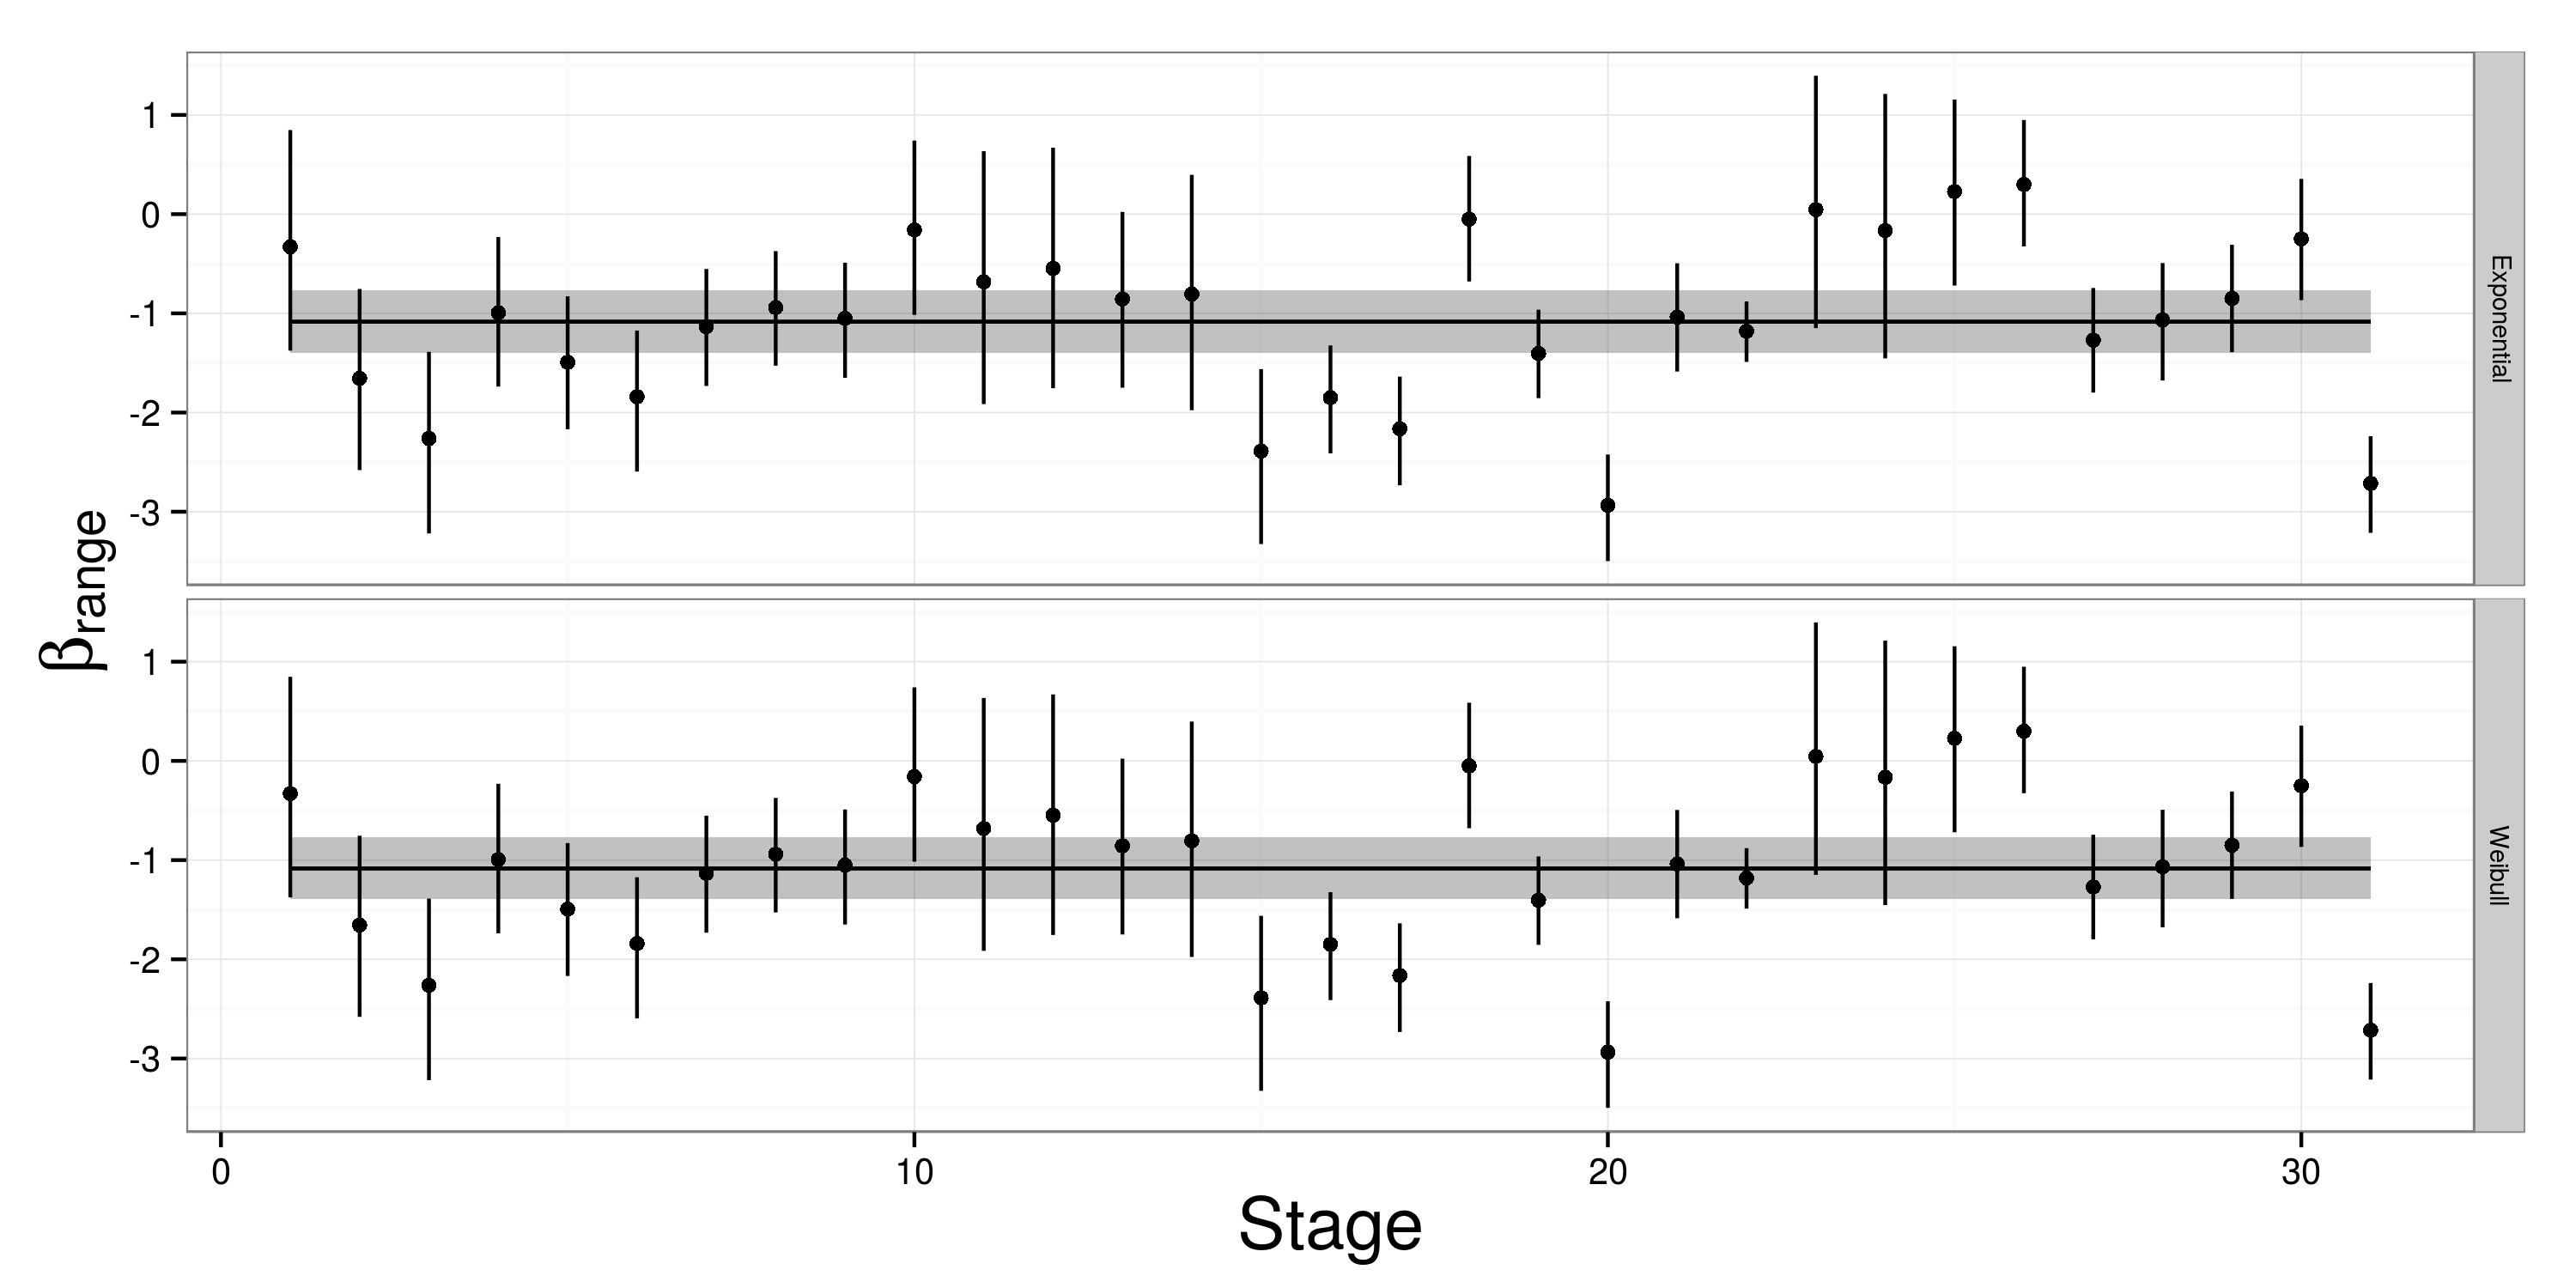
\includegraphics[height = 0.5\textheight,width=\textwidth,keepaspectratio=true]{figure/range_cohort}
  \caption{<+caption text+>}
  \label{fig:cohort_range}
\end{figure}

% environmental effect for cohort
%   effect of environmental preference as duration multiplier
How the effect of environmental affinity varies between cohorts can be observed by using the cohort specific coefficients estimates. Following the exact same procedure used earlier (Fig. \ref{fig:tau}), but substituting cohort specific estimates of \(\beta_{v}\) and \(\beta_{v^{2}}\) for \(\mu_{v}\) and \(\mu_{v^{2}}\), the cohort specific effect of environmental preference as a multiplier of mean extinction risk can be calculated. This was done only for the Weibull model, though the observed pattern should be similar for the exponential model. 

As expected based on the estimates of \(\tau_{v}\) and \(\tau_{v^{2}}\), there is greater variation in the peakedness of \(f(v_{i}\) than there is variation between upward and downward facing functions (Fig. \ref{fig:env_cohort}). Only 9 of the 31 cohorts have less than 50\% posterior probability that generalists are shorter lived than specialists, though 2 of those cases have approximately a 50\% probability of being either upward or downward facing. This is congruent with the 0.70+ posterior probability that \(\mu_{v^{2}}\) is positive/\(f(v_{i})\) is downward facing, which corresponds to approximately 8 out of 31 cohorts.

Additionally, a quite striking pattern emerges when the inflection point of the function is either far away from the y-intercept (x = 0, y = 1) or when there is little evidence of non-linearity (Fig. \ref{fig:env_cohort}). Cohort 21 and 20, for example, have almost linear relationships between environmental preference and the duration multiplier. This type of relationship occurs when \(\beta_{v^{2}}\) approaches 0, flattening the non-linear curvature of the relationship.

\begin{sidewaysfigure}[ht]
  \centering
  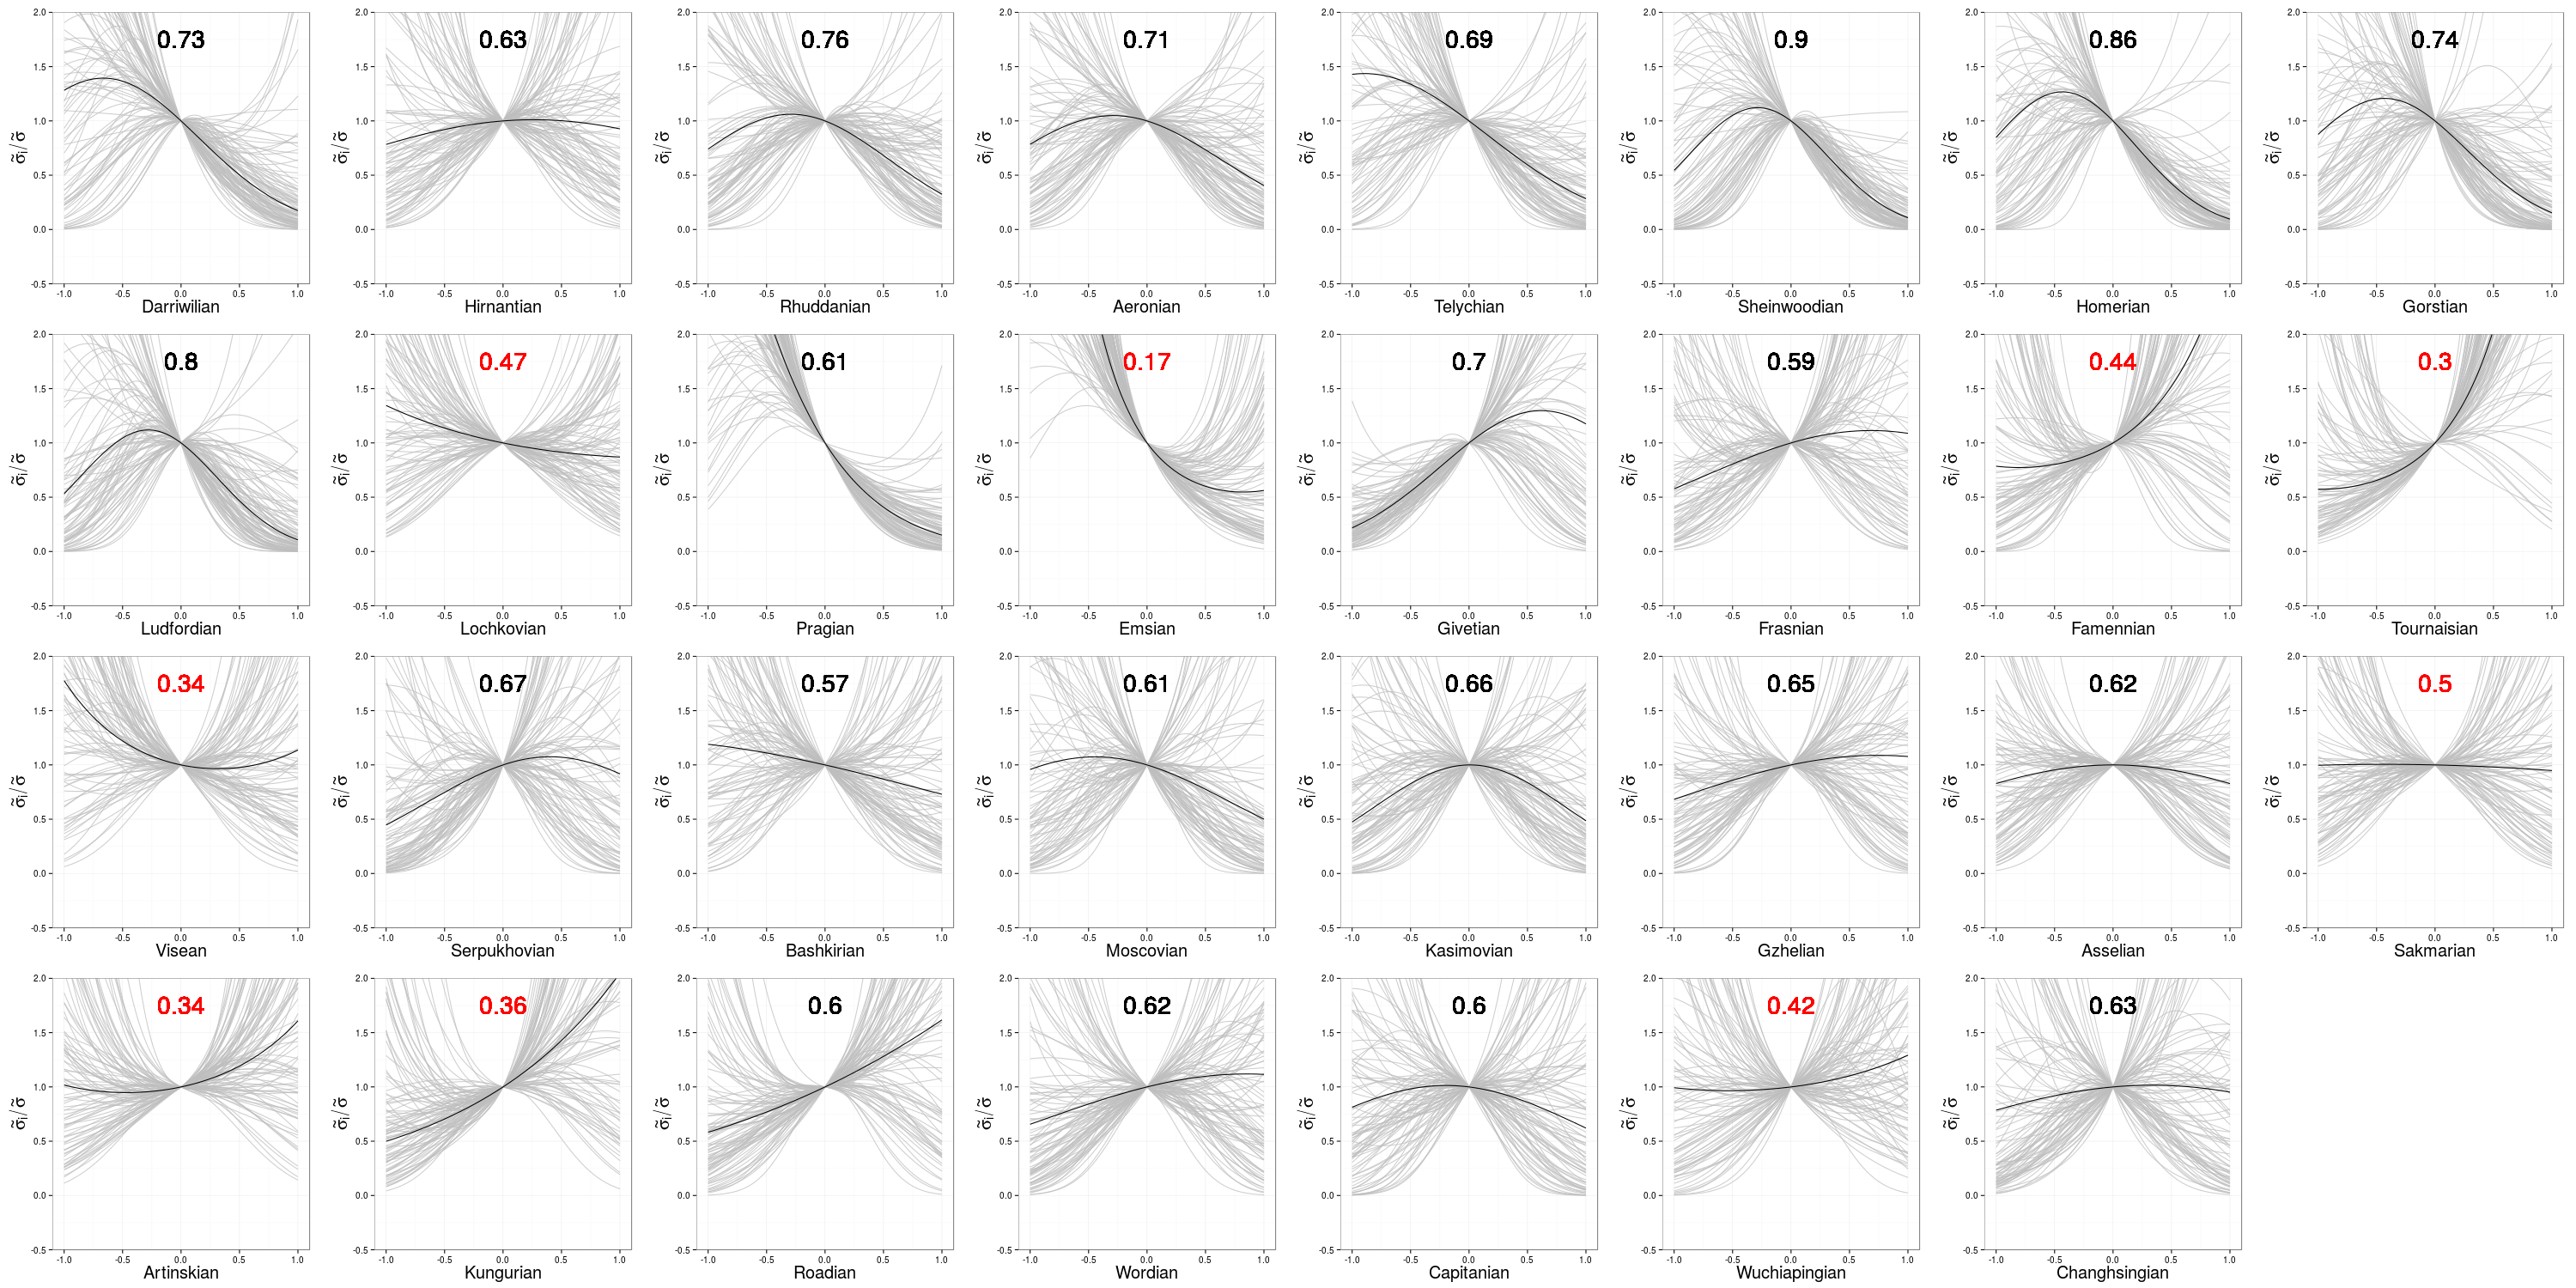
\includegraphics[height = 0.5\textheight,width=\textwidth,keepaspectratio=true]{figure/cohort_quads}
  \caption{<+caption text+>}
  \label{fig:env_cohort}
\end{sidewaysfigure}


\end{document}


\documentclass[12pt,letterpaper]{article}

\usepackage{amsmath, amsthm}
\usepackage{microtype, parskip}
\usepackage[comma,numbers,sort&compress]{natbib}
\usepackage{lineno}
\usepackage{docmute}
\usepackage{caption, subcaption, multirow, morefloats, rotating}
\usepackage{wrapfig}

\frenchspacing

\captionsetup[subfigure]{position = top, labelfont = bf, textfont = normalfont, singlelinecheck = off, justification = raggedright}

\begin{document}
\section{Discussion}

% hypotheses
%   Jablonski1986 hypothesis
My results demonstrate that both the effects of geographic range and the peakedness/concavity of environmental preference are both negatively correlated with baseline extinction risk, meaning that as baseline extinction risk increases the effect sizes of both these traits are expected to increase (Fig. \ref{fig:corr}). This result supports neither of the two proposed macroevolutionary mechanisms for how biological traits should correlate with extinction risk. The observed correlation between the two effects as well as between the effects and baseline extinction risk instead implies that as baseline extinction risk increases, the strength of the total selection gradient on biological traits (except body size) increases. This manifests as greater differences in extinction risk for each unit difference in the biological covariates during periods of high extinction risk, while a relatively flater selection gradient during periods of low extinction risk.

%   Miller2009a results
There are two mass extinction events that are captured within the time frame considered here: the Ordovician-Silurian and the Frasnaian-Famennian. The cohorts bracketing these events are worth considering in more detail.

% write about the mass extinctions \ref{fig:env_cohort}

The proposed mechanism for the end Ordovician mass extinction is a decrease in sea level and the draining of epicontinental seas due to protracted glaciation \citep{Sheehan2001b,Johnson1974}. My results are broadly consistent with this scenario with both epicontinental and open-ocean specialists having a much lower expected duration than intermediate taxa (Fig. \ref{fig:env_cohort}). All of the stages between the Darriwillian and the Llandovery, except the Hirnantian, have a greater than expected probability that \(f(v)\) is concave down. The pattern for the Darriwilian, which marks the supposed start of Ordovician glacial activity, demonstrates that taxa tend to favor open-ocean environments are expected to have a greater duration than either intermediate of epicontinental specialists, in decreasing order.

For nearly the entire Devonian estimates of \(f(v)\) indicate that one of the environmental end members is favored over the other end member of intermediate preference (Fig. \ref{fig:env_cohort}). This is consistent with \citet{Miller2009a}. For the Givetian though the end of the Devonian and into the Tournasisian, I find that epicontinental favoring taxa are expected to have a greater duration than either intermediate or open-ocean specialists. Additionally, for nearly the entire Devonian except the Eifelian and through the Visean, the cohort-specific estimates of \(f(v)\) are concave-up. This is the opposite pattern than what is expected (Fig. \ref{fig:env_mean}). This result, however, seems to reflect the intensity of the seemingly nearly-linear difference in expected duration across the range of \(v)\) as opposed to an inversion of the weakly expected curvilinear pattern.

There is an approximate 86\% posterior probability that taxa with intermediate environmental preferences are possibly expected to have a lesser extinction risk than either end members, the over all curvature of \(f(v_{i})\) is not very peaked, meaning that this relationship does not lead to very strong differences in extinction risk (Fig. \ref{fig:env_mean}). This result gives weak support for the hypothesis that, in general, environmental generalists survive for longer than environmental specialists \citep{Simpson1944,Liow2004a,Liow2007b,Nurnberg2013a,Nurnberg2015}.

The variance in estimate of the overall \(f(v_{i})\) reflects the large between cohort variance in cohort specific estimates of \(f(v_{i})\) (Fig. \ref{fig:env_cohort}). Given that there is only a 86\% posterior probability that the expected overall estimate of \(f(v_{i})\) is concave down, it is not surprising that there are some stages where the theorized relationship is in fact reversed. Additionally, as discussed earlier, some of those same stages where \(f(v_{i})\) does not resemble the theorized nonlinear relation with the optimum in the middle, but are instead is highly skewed or effectively linear (Fig. \ref{fig:env_cohort}). 

These results do not necessarily refute ``survival of the unspecialized'' as a time-invariant generalization, but instead demonstrate how, while the expected group-level estimate of \(f(v_{i})\) might favor one hypothesis, there is still enough variability between cohorts so that in some realizations this pattern may not hold or can even be reversed. These results are also consistent with aspects of \citet{Miller2009a} who found that the effect of environmental preference on extinction risk was quite variable and without obvious patterning during times of background extinction.

% defense
%   species:genus?
%   difficulty towards tails, but that's to be expected
%     this model is about expectations, not tails/extreme events
%     this model is ok for the main part of the data
%     though, of course, this model has a long way to go (all models are false)

% future direction
This model can be improved through either increasing the number of analyzed taxon traits, expanding the hierarchical structure of the model to include other major taxonomic groups of interest, and the inclusion of explicit phylogenetic relationships between the taxa in the model as an additional hierarchical effect.

%   other measures of ecology? affixing strategy a la Alexander1977
An example taxon trait that may be of particular interest is the affixing strategy or method of interaction with the substrate of the taxon. This trait has been found to be related to brachiopod survival \citep{Alexander1977} so its inclusion may be of particular interest.

%   comparison with other major groups in hierarchical model
It is theoretically possible to expand this model to allow for comparisons within and between major taxonomic groups. This approach would better constrain the brachiopod estimates while also allowing for estimation of similarities and differences in cross-taxonomic patterns. The major issue surrounding this particular expansion involves finding an similarly well sampled taxonomic group that is present during the Paleozoic. Example groups include Crinoidea, Ostracoda, and other ``Paleozoic'' groups \citep{SepkoskiJr.1981a}.

%   integration of phylogenetic information/taxonomic component
%     taxon traits are more than likely heritable
%     what aspect of variation is explained just by 
%     see Smits Submitted
Taxon traits like environmental preference or geographic range \citep{Jablonski1987,Hunt2005b} are most likely heritable, at least phylogenetically \citep{Lynch1991,Housworth2004}. Without phylogenetic context, this analysis assumes that differences in extinction risk between taxa are independent of those taxa's shared evolutionary history \citep{Felsenstein1985b}. In contrast, the origination cohorts only capture shared temporal context. The inclusion of phylogenetic context as an addition individual level hierarchical structure independent of origination cohort would allow for determining how much of the observed variability is due to shared evolutionary history versus actual differences associated with these taxonomic traits. For example, it has been shown that phylogeny contribute non-trivially to differences in mammal species durations \uppercase{Smits in prep}.

% concluding statements
In summary, patterns of Paleozoic brachiopod survival were analyzed using a fully Bayesian hierarchical survival modelling approach. Using a varying-slopes, varying-intercepts approach I am able to model both the overall mean effect of biological covariates on extinction risk while also modeling the correlation between origination cohort-specific estimates of covariate effects. I find that as baseline extinction risk increases, the strength of the selection gradient on biological traits (except body size) increases. This manifests as greater differences in extinction risk for each unit difference in the biological covariates during periods of high extinction risk, while a much flatter total selection gradient during periods of low extinction risk. I also find some support for ``survival of the unspecialized'' \citep{Simpson1944,Liow2004a,Liow2007b,Nurnberg2013a,Nurnberg2015} as a general characterization of the effect of environmental preference on extinction risk (Fig. \ref{fig:env_mean}), though there is heterogeneity between origination cohorts (Fig. \ref{fig:env_cohort}). Generally, this study demonstrates the advantages of a hierarchical Bayesian framework for taking into account the structured nature of the data. Future studies of structured data should adopt similar strategies in order to best model our knowledge instead of ignoring that structure which can lead to poor and/or incorrect inference.

\end{document}


\section*{Acknowledgements}
I would like to thank K. Angielzcyk, M. Foote, P. D. Polly, and R. Ree for helpful discussion and advice. Additionally, thank you A. Miller for the epicontinental versus open-ocean assignments. This entire study would would not have been possible without the Herculean effort of the many contributors to the Paleobiology Database. In particular, I would like to thank J. Alroy, M. Aberhan, D. Bottjer, M. Clapham, F. F\"{u}rsich, N. Heim, A. Hendy, S. Holland, L. Ivany, W. Kiessling, B. Kr\"{o}ger, A. McGowan, T. Olszewski, P. Novack-Gottshall, M. Patzkowsky, M. Uhen, L. Villier, and P. Wager. This work was supported by a NASA Exobiology grant (NNX10AQ446) to M. Foote and A. Miller. This is Paleobiology Database publication XXX.

\clearpage

\bibliographystyle{evolution}
\bibliography{newbib,packages}

\clearpage

\appendix
\documentclass[12pt,letterpaper]{article}

\usepackage{amsmath, amsthm}
\usepackage{microtype, parskip}
\usepackage[comma,numbers,sort&compress]{natbib}
\usepackage{lineno}
\usepackage{docmute}
\usepackage{caption, subcaption, multirow, morefloats, rotating}
\usepackage{wrapfig}

\frenchspacing

\captionsetup[subfigure]{position = top, labelfont = bf, textfont = normalfont, singlelinecheck = off, justification = raggedright}

\begin{document}
\section{Uncertainty in environmental preference} \label{sec:uncer}
The calculation and inclusion of environmental affinity in the survival model is a statistical procedure that takes into account our uncertainty based on where fossils tend to occur. Because we cannot directly observe if a fossil taxon had occurrences restricted to only a single environment, instead we can only estimate its affinity with uncertainty. One advantage of using a Bayesian analytical approach is that both parameters and data are considered random samples from some underlying distribution, which means that is is possible to model the uncertainty in our covariates of interest \citep{Gelman2013d}. My approach is conceptually similar to \citet{Simpson2009} but instead of obtaining a single point estimate, an entire posterior distribution is estimated.

The first step is to determine the probability \(\theta\) at which genus \(i\) occurs in an epicontinental settings based on its own pattern of occurrences. Define \(e_{i}\) as the number of occurrences of genus \(i\) in an epicontiental sea and \(o_{i}\) as the number of occurrences of genus \(i\) not in an epicontinental sea (e.g. open ocean). Because the value of interest is the probability of occurring in an epicontinental environment, given the observed fossil record, I assume that probability follows a binomial distribution. We can then define our sampling statement as
\begin{equation}
  e_{i} \sim \mathrm{Binomial}(e_{i} + o_{i}, \theta_{i}).
  \label{eq:epi_lik}
\end{equation}
I used a flat prior for \(\theta_{i}\) defined as \(\theta_{i} \sim \mathrm{Beta}(1, 1)\). Because the beta distribution is the conjugate prior for the binomial distribution, the posterior is easy to compute in closed form. The posterior probability of \(\theta\) is then 
\begin{equation}
  \theta_{i} \sim \mathrm{Beta}(e_{i} + 1, o_{i} + 1)
  \label{eq:epi_post}
\end{equation}

It is extremely important, however, to take into account the overall environmental occurrence probability of all other genera present at the same time as genus \(i\). This is incorporated as an additional probability \(\Theta\). Define \(E_{i}\) as the total number of other fossil occurrences (exceptfor genus \(i\)) in epicontinental seas during stages where \(i\) occurs and \(O_{i}\) as the number of other fossil occurrences not on epicontinental seas. We can then define the sampling statement as
\begin{equation}
  E_{i} \sim \mathrm{Binomial}(E_{i} + O_{i}, \Theta_{i}).
  \label{eq:bck_lik}
\end{equation}
Again, I used a flat prior of \(\Theta_{i}\) defined as \(\Theta_{i} \sim \mathrm{Beta}(1, 1)\). The posterior of \(\Theta\) is then simply defined as

\begin{equation}
  \Theta_{i} \sim \mathrm{Beta}(E_{i} + 1, O_{i} + 1)
  \label{eq:bck_post}
\end{equation}

I then define the environmental affinity of genus \(i\) as \(v_{i} = \theta_{i} - \Theta_{i}\). \(v_{i}\) is a value that can range between -1 and 1, where negative values indicate that genus \(i\) tends to occur more frequently in open ocean environments than background while positive values indicate that genus \(i\) tends to occur in epicontiental environments.

While this approach is noticeably more complicated than previous ones \citep{Foote2006,Miller2001,Simpson2009,Kiessling2007a} there are some important benefits to both using a continuous measure of affinity as well directly modeling our uncertainty. In order to show some of these benefits, I performed a simulation analysis of how modal/maximum \textit{a posteriori} (MAP) estimates versus full posterior estimates.

In this simulation, I first defined the ``background'' epicontinental occurrence \(\theta_{b}\) as 0.50 with a small amount of noise. This was represented as a beta distribution 

\begin{equation}
  \Theta_{b} = \mathrm{Beta}(\alpha = 2500, \beta = 2500). 
  \label{eq:bck_sim}
\end{equation}
This choice of parameters for the distribution reflects the average number of background occurrences for either epicontinental or open ocean environments per genus.

Using this background occurrence ratio, I randomly generated the occurrence patterns of 1000 simulated taxa. This was done at multiple sample sizes (1, 2, 3, 4, 5, 10, 25, 50, 100) in order to demonstrate the effects of increasing sample size on the confidence of environmental affinity. For each simulated taxon I calculated the full posterior distribution while assuming a flat Beta prior (\(\mathrm{Beta}(1, 1)\)). Using the full posterior I calculated the MAP probability of occurring in epicontinental environments. The environmental affinity was calculated for each of the simulated taxa using both the full posterior and the MAP estimate. In this toy example, environmental affinity can range between -0.5 and 0.5.

As should be expected, as sample size increases the distribution of MAP estimates converge on the true value (Fig. \ref{fig:env_mode}). For taxa with less than 10 occurrences, the MAP estimate is biased towards extreme values. Note that the mode of the beta distribution is not defined for situations where there were 0 draws of one of the environmental conditions. Instead, the vertical line is based entirely on the observed occurrences which are technically the modal estimates because they are the most frequently occurring/highest density.

In contrast, we can compare the true occurrence probability distribution versus the posterior estimate for a given sample (Fig. \ref{fig:env_post}). When sample sizes are low, posterior estimates are flat and represent a compromise between the likelihood and the flat prior (Eq. \ref{eq:epi_post}). Because of this, estimates from small sizes are less likely to be overly biased towards the extremes. This is further emphasized by inspection of the estimates of environmental affinity for the simulated taxa (Fig. \ref{fig:env_diff}). Posterior estimates from simulated taxa with small sample size have a much broader distribution that both allows for the extreme observation but still captures the ``true'' value (0). 


By defining environmental preference as the difference in full posterior estimates of occurrence probability, it is possible to include taxa with low sample sizes that are normal discarded \citep{Foote2006,Miller2001,Simpson2009,Kiessling2007a}. Additionally, 55+\% of observed Paleozoic brachiopod genera have less than 10 occurrences which is the range of sample sizes where MAP (or ML) estimates would be potentially most biased. This is preferable to finding the difference between the MAP estimates (blue line; Fig. \ref{fig:env_diff}).

% behavior of MAP estimates
%   as sample size increases, converge on true (10+)
% behavior of posterior
%   compromise between likelihood of data occurrences and (flat) prior
%   really important for small sample sizes
%   at 10+ makes no difference anymore
%   this is also kind obvious from the estimates of \(v\)
% how many taxa have less than 10 occurrences? \approx 55\%

\begin{figure}[ht]
  \centering
  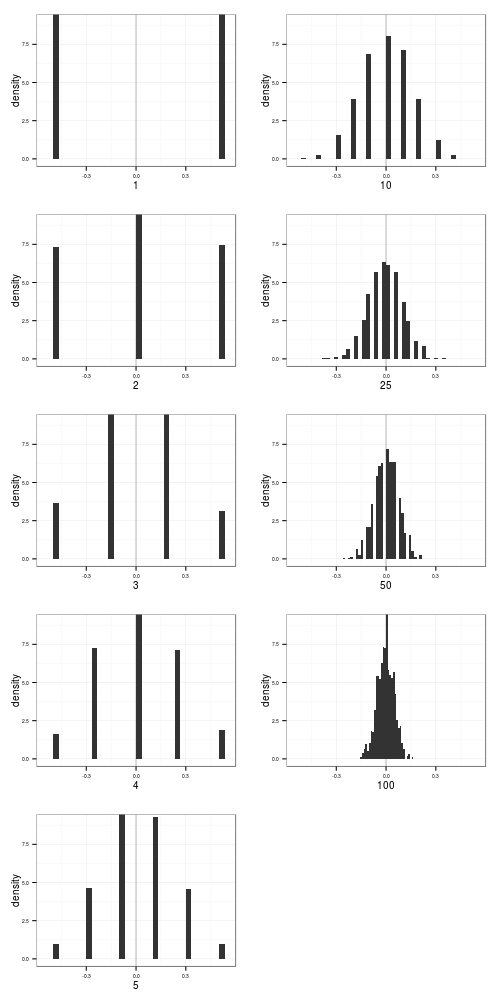
\includegraphics[height = \textheight,width=\textwidth,keepaspectratio=true]{figure/env_mode_dist}
  \caption{Histograms of the distributions of from the beta distribution defined in Eq. \ref{eq:bck_sim}. As to be expected, as sample size increases the draws better resemble the underlying true distribution. Sample size is indicated as the label of the x-axis, increasing in column major order.}
  \label{fig:env_mode}
\end{figure}

\begin{figure}[ht]
  \centering
  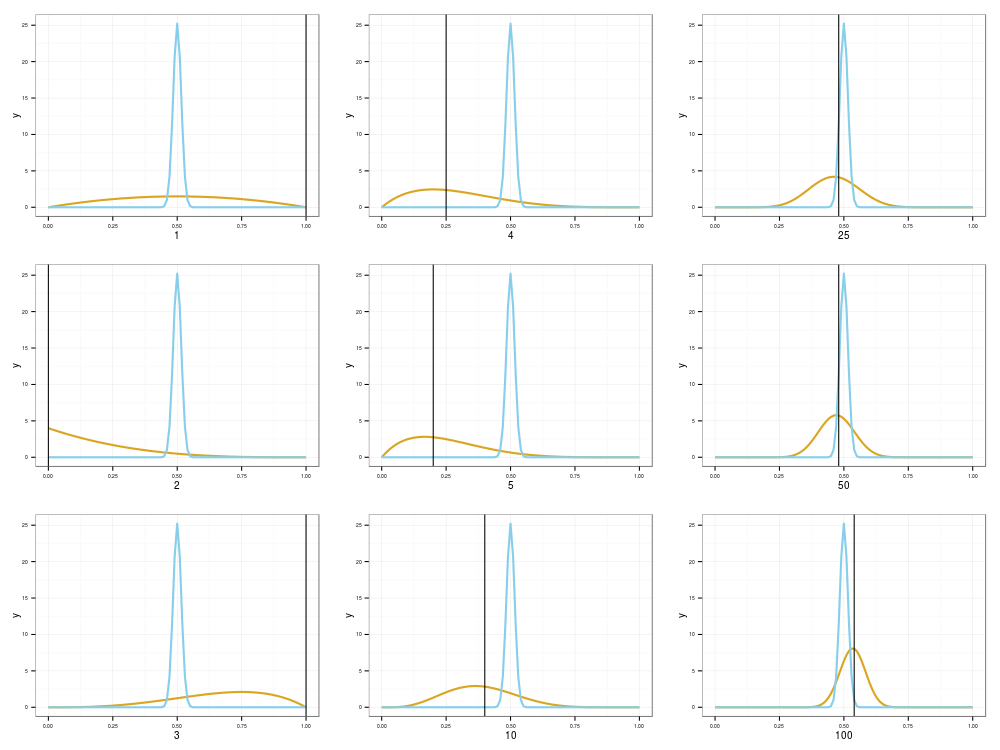
\includegraphics[height = \textheight,width=\textwidth,keepaspectratio=true]{figure/env_post_inspect}
  \caption{Comparisons of the underlying distribution (blue) to posterior estimates based on increasing sample size (gold). Each posterior estimate is represented for only a single realization of draws, each with sample size indicated as the x-axis label (increasing in column major order). Black vertical lines correspond to the MAP estimate of the simulated taxon's affinity. This stands in contrast to the posterior distribution of expected affinity in gold.}
  \label{fig:env_post}
\end{figure}

\begin{figure}[ht]
  \centering
  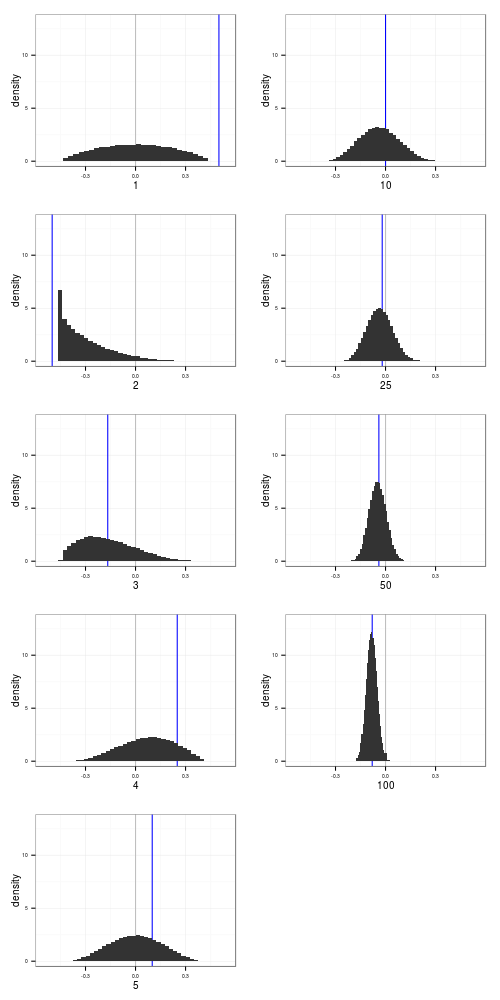
\includegraphics[height = \textheight,width=\textwidth,keepaspectratio=true]{figure/env_diff}
  \caption{Histograms of the difference in the underlying occurrence distribution and the posterior distribution estimates from the previous graph (Fig. \ref{fig:env_post}). The ``true'' value is included in all distributions of environmental affinities. Each affinity estimate is represented for only a single realization of draws, each with sample size indicated as the x-axis label (increasing in column major order). Blue vertical lines correspond to the difference in MAP estimates between the underlying distribution and the simulated taxon's draws. This stands in contrast to the distribution of the differences between the simulated taxon and background.}
  \label{fig:env_diff}
\end{figure}

\section{Survival model} \label{sec:survival}

The simplest model of genus duration includes no covariate or structural information. Define \(y_{i}\) as the duration in stages of genus \(i\), where \(i = 1, \dots, n\) and \(n\) is the number of observed genera. These two models are them simply defined as
\begin{equation}
  \begin{aligned}
    y_{i} &\sim \mathrm{Exponential}(\lambda) \\
    y_{i} &\sim \mathrm{Weibull}(\alpha, \sigma).
  \end{aligned}
  \label{eq:simple}
\end{equation}
\(\lambda, \alpha, \text{and} \sigma\) are all defined for all positive reals. Note that \(\lambda\) is a ``rate'' or inverse-scale while \(\sigma\) is a scale parameter, meaning that \(\frac{1}{\lambda} = \sigma\).

These simple models can then be expanded to include covariate information as predictors by reparameterizing \(\lambda\) or \(\sigma\) as a regression \citep{Klein2003}. Each of the covariates of interest is given its own regression coefficient (e.g. \(\beta_{r}\)) along with an intercept term \(\beta_{0}\). There are some additional complications to the parameterization of \(\sigma\) associated with the inclusion of \(\alpha\) as well as for interpretability \citep{Klein2003}. Both of these are then written as
\begin{equation}
  \begin{aligned}
    \lambda_{i} &= \exp(\beta_{0} + \beta_{r} r_{i} + \beta_{v} v_{i} + \beta_{v^{2}} v_{i}^{2} + \beta_{m} m_{i}) \\
    \sigma_{i} &= \exp\left(\frac{-(\beta_{0} + \beta_{r} r_{i} + \beta_{v} v_{i} + \beta_{v^{2}} v_{i}^{2} + \beta_{m} m_{i})}{\alpha}\right).
  \end{aligned}
  \label{eq:regression}
\end{equation}
The quadratic term for environmental affinity \(v\) is to allow for the possible nonlinear relationship between environmental affinity and extinction risk.

The models which incorporate both equations \ref{eq:simple} and \ref{eq:regression} can then be further expanded to allow all of the \(\beta\) coefficients, including \(\beta_{0}\), to vary with origination cohort while also modeling their covariance and correlation. This is called a varying-intercepts, varying-slopes model \citep{Gelman2007}. It is much easier to represent and explain how this is parameterized using matrix notation. First, define \(\mathbf{B}\) as \(k \times J\) matrix of the \(k\) coefficients including the intercept term (\(k = 5\)) for each of the \(J\) cohorts. Second, define \(\mathbf{X}\) as a \(n \times k\) matrix where each column is one of the covariates of interest. Importantly, \(\mathbf{X}\) includes a columns of all 1s which correspond to the constant term \(\beta_{0}\). Third, define \(j[i]\) as the origination cohort of genus \(i\), where \(j = 1, \dots, J\) and \(J\) is the total number of observed cohorts. We then rewrite \(\lambda\) and \(\sigma\) of equation \ref{eq:regression} in matrix notation as
\begin{equation}
  \begin{aligned}
    \lambda_{i} &= \exp(\mathbf{X}_{i} B_{j[i]}) \\
    \sigma_{i} &= \exp\left(\frac{-(\mathbf{X}_{i} B_{j[i]})}{\alpha}\right). 
  \end{aligned}
  \label{eq:multivariate}
\end{equation}

Because \(B\) is a matrix, I use a multivariate normal prior with unknown vector of means \(\mu\) and covariance matrix \(\Sigma\). This is written as 
\begin{equation}
  B \sim \mathrm{MVN}(\vec{\mu}, \Sigma)
  \label{eq:beta_prior}
\end{equation}
where \(\vec{\mu}\) is length \(k\) vector representing the overall mean of the distributions of \(\beta\) coefficients. \(\Sigma\) is a \(k \times k\) covariance matrix of the \(\beta\) coefficients.

What remains is assigning priors the elements of \(\vec{\mu}\) and the covariance matrix \(\Sigma\). All elements of \(\vec{\mu}\) except for \(\mu_{r}\) were given horseshoe priors \citep{Carvalho2010,Carvalho2009} while \(\mu_{r}\) was given an informative normal prior (\(\mu_{r} \sim \mathcal{N}(-1, 1)\). Horseshoe priors are a strong regularizing priors with effectively infinite density at 0 and heavy, Cauchy-like tails \citep{Carvalho2010,Carvalho2009} which allow weakly inferred effects to be strongly drawn towards 0 while truly strong effects can remain large. The horseshoe prior consists of a normal distribution with scale term that is the product between a global shrinkage parameter \(\nu\) and a locak shrinkage parameter \(\psi\) unique to each of the parameters of interest. These parameters are themselves given half-Cauchy priors (Eq. \ref{eq:exp_total} and \ref{eq:wei_total}).

The prior for \(\Sigma\) is a bit more complicated due to its multivariate nature. Following the \citet{stan-manual:2014}, I modeled the scale terms separate from the correlation structure of the coefficients. This is possible because of the relationship between a covariance and a correlation matrix, defined as 
\begin{equation}
  \Sigma_{B} = \text{Diag}(\vec{\tau}) \Omega \text{Diag}(\vec{\tau})
  \label{eq:covcor}
\end{equation}
where \(\vec{\tau}\) is a length \(k\) vector of variances and Diag(\(\tau\)) is a diagonal matrix.

I used a LKJ prior distribution for correlation matrix \(\Omega\) as recommended by \citet{stan-manual:2014}. The LKJ distribution is a single parameter multivariate distribution where values of the parameter \(\eta\) greater than 1 concentrate density at the unit correlation matrix, which corresponds to no correlation between the \(\beta\) coefficients. The scale parameters, \(\vec{\tau}\), are given weakly informative half-Cauchy (C\(^{+}\)) priors following \citet{Gelman2006a}.



\section{Censored observations} \label{sec:cen}
A key aspect of survival analysis is the inclusion of censored, or incompletely observed, data points \citep{Ibrahim2001,Klein2003}. The two classes of censored observations encountered in this study were right and left censored observations. Right censored genera are those that did not go extinct during the window of observation, or genera that are still extant. Left censored observations are those taxa for which we know only an upper limit on their duration.

In the context of this study, I considered all genera that had a duration of only one geologic stage to be left censored as we do not have a finer degree of resolution. 

The key function for modeling censored observations is the survival function, or \(S(t)\). \(S(t)\) corresponds to the probability that a genus having existed for \(t\) stages will not have gone extinct while \(h(t)\) corresponds to the instantaneous extinction rate at taxon age \(t\) \cite{Klein2003}. For an exponential model, \(S(t)\) is defined as
\begin{equation}
  S(t) = \exp(-\lambda t),
  \label{eq:exp_surv}
\end{equation}
and for the Weibull distribution \(S(t)\) is defined as
\begin{equation}
  S(t) = \exp\left(-\left(\frac{t}{\sigma}\right)^{\alpha}\right).
  \label{eq:wei_surv}
\end{equation}
\(S(t)\) is equivalent to the complementary cumulative distribution function, \(1 - F(t)\) \citep{Klein2003}. 

For right censored observations, instead of calculating the likelihood as normal (Eq. \ref{eq:multivariate}) the likelihood of an observation is evaluated using \(S(t)\). Conceptually, this approach calculates the likelihood of observing a taxon that existed for at least that long. For left censored data, instead the likelihood is calculated using \(1 - S(t)\) which corresponds to the likelihood of observing a taxon that existed no longer than \(t\).

The full likelihood statements incorporating fully observed, right censored, and left censored observations are then
\begin{equation}
  \begin{aligned}
    \mathcal{L} &\propto \prod_{i \in C} \mathrm{Exponential}(y_{i} | \lambda) \prod_{j \in R} S(y_{j} | \lambda) \prod_{k \in L} \left(1 - S(y_{k} | \lambda)\right) \\
    \mathcal{L} &\propto \prod_{i \in C} \mathrm{Weibull}(y_{i} | \alpha, \sigma) \prod_{j \in R} S(y_{j} | \alpha, \sigma) \prod_{k \in L} \left(1 - S(y_{k} | \alpha, \sigma)\right)
  \end{aligned}
  \label{eq:censored_likelihood}
\end{equation}
where \(C\) is the set of all fully observed taxa, \(R\) the set of all right censored taxa, and \(L\) the set of all left-censored taxa.


\section{Widely applicable information criterion} \label{sec:waic}
WAIC can be considered a fully Bayesian alternative to the Akaike information criterion, where WAIC acts as an approximation of leave-one-out cross-validation which acts as a measure of out-of-sample predictive accuracy \citep{Gelman2013d}. WAIC is calculated starting with the log pointwise posterior predictive density calculated as
\begin{equation}
  \mathrm{lppd} = \sum_{i = 1}^{n} \log \left(\frac{1}{S} \sum_{s = 1}^{S} p(y_{i}|\Theta^{S})\right),
  \label{eq:lppd}
\end{equation}
where \(n\) is sample size, \(S\) is the number posterior simulation draws, and \(\Theta\) represents all of the estimated parameters of the model. This is similar to calculating the likelihood of each observation given the entire posterior. A correction for the effective number of parameters is then added to lppd to adjust for overfitting. The effective number of parameters is calculated, following the recommendations of \citet{Gelman2013d}, as
\begin{equation}
  p_{\mathrm{WAIC}} = \sum_{i = 1}^{n} V_{s = 1}^{S} (\log p(y_{i}|\Theta^{S})).
  \label{eq:pwaic}
\end{equation}
where \(V\) is the sample posterior variance of the log predictive density for each data point.

Given both equations \ref{eq:lppd} and \ref{eq:pwaic}, WAIC is then calculated
\begin{equation}
  \mathrm{WAIC} = \mathrm{lppd} - p_{\mathrm{WAIC}}.
  \label{eq:waic}
\end{equation}
When comparing two or more models, lower WAIC values indicate better out-of-sample predictive accuracy. Importantly, WAIC is just one way of comparing models. When combined with posterior predictive checks it is possible to get a more complete understanding of a model's fit to the data.

\end{document}


\end{document}
